\documentclass[11pt,a4paper]{article}

\usepackage[margin=2.3cm]{geometry}
\usepackage[utf8]{inputenc}
\usepackage[T1]{fontenc}
\usepackage{booktabs}
\usepackage{array}
\usepackage{longtable}
\usepackage{graphicx}
\usepackage{xcolor}
\usepackage{caption}
\usepackage{subcaption}
\usepackage{amsmath}
\usepackage{enumitem}
\usepackage[colorlinks=true,linkcolor=blue,citecolor=blue,urlcolor=blue]{hyperref}
\usepackage{microtype}
\sloppy

\newcommand{\code}[1]{\texttt{#1}}
\newcolumntype{R}[1]{>{\raggedleft\arraybackslash}p{#1}}

\title{\textbf{Cross-Country PII Exposure and Risk Analysis}\\
\large A synthesis of storage-level privacy findings for thirteen country personas}
\author{PII Statistical Modeling -- Country Extension}
\date{\today}

\begin{document}
\maketitle

\begin{abstract}
\noindent
This document synthesizes the results of the country-level extension of the PII
statistical modeling pipeline, covering thirteen synthetic personas
(\code{IT\_0573}, \code{LU\_0634}, \code{PT\_0838}, \code{SE\_0964}, \code{ES\_0290}, \code{DE\_0018}, \code{FR\_0429}, \code{IE\_0504}, \code{NL\_0694}, \code{PL\_0742}, \code{AT\_0077}, \code{DK\_0199}, \code{FI\_0373}) browsing under two authentication states
(\code{AUTH} / \code{NOTAUTH}) with a single consent policy
(\code{PARTIAL}, labeled \emph{Essential Only} in the figures below). It covers data
volumes, PII category prevalence, storage-type distribution, cookie security
non-conformity, and the exposure--impact--risk ($P_i \times I_i = R_i$) scoring
model, and closes with an explicit discussion of the methodology's accuracy
and limitations. The country pipeline is fully separate from the original
three-user French (FR) pipeline; no FR script, data, or published result was
modified in the course of this work. This revision extends an earlier
six-country version of the same report with seven additional personas
(\code{FR\_0429}, \code{IE\_0504}, \code{NL\_0694}, \code{PL\_0742},
\code{AT\_0077}, \code{DK\_0199}, \code{FI\_0373}); every number below is
recomputed from the full thirteen-country dataset, not merged with the earlier figures.
\end{abstract}

\tableofcontents

% ============================================================
\section{Introduction and Scope}
% ============================================================

The goal of this analysis is to compare how much personal data, of what kind,
and under what technical protection, is collected by websites across
thirteen country contexts, and whether authentication status changes that
exposure. Each persona is a synthetic identity (\emph{Chris Martin}) carrying
country-specific contact details, browsing a set of country-appropriate sites
while their browser's cookies, \code{localStorage}, \code{sessionStorage}, and
\code{IndexedDB} stores were captured.

\begin{table}[h]
\centering
\caption{Scope of the country dataset.}
\begin{tabular}{lp{10.5cm}}
\toprule
Dimension & Value \\
\midrule
Countries (personas) & \code{IT\_0573}, \code{LU\_0634}, \code{PT\_0838}, \code{SE\_0964}, \code{ES\_0290}, \code{DE\_0018}, \code{FR\_0429}, \code{IE\_0504}, \code{NL\_0694}, \code{PL\_0742}, \code{AT\_0077}, \code{DK\_0199}, \code{FI\_0373} \\
Authentication states & AUTH, NOTAUTH \\
Consent policy & PARTIAL / ``Essential Only'' (only) \\
Storage types & cookies, localStorage, sessionStorage, IndexedDB \\
Lifecycle events tracked & added, modified, removed \\
Profiles analyzed & 26 (13 countries $\times$ 2 auth states) \\
\bottomrule
\end{tabular}
\end{table}

Unlike the original French dataset -- which was collected under three consent
policies (\code{ALL}/\code{PARTIAL}/\code{NONE}) -- the country dataset only
has \code{PARTIAL}. Consequently, every comparison that in the FR pipeline ran
across consent policies has no equivalent here; this document instead adds a
comparison axis the FR pipeline never had: side-by-side comparison across the
thirteen countries themselves.

% ============================================================
\section{Methodology Overview}
% ============================================================

The pipeline runs in three stages, each fully separated from the FR pipeline
by directory (no FR script or output is read or written by any stage below).

\begin{enumerate}[label=\textbf{Stage \arabic*.}, leftmargin=2.2cm]
  \item \textbf{Categorization.} Raw captures are labeled into PII categories
    (e.g. \code{DIRECT\_PII}, \code{BEHAVIORAL\_DATA}, \code{IDENTITY\_TRACKING})
    first by regex matching against the personas' known ground-truth identity
    fields and generic tracking-keyword patterns, then by an LLM
    (\code{gpt-4.1-mini}) pass over whatever regex left \code{UNCATEGORIZED},
    followed by a dedicated correction pass and a final hand-audited regex
    pass for third-party SDK field-naming schemes.
  \item \textbf{Descriptive analysis.} Category prevalence, storage-type
    breakdown, cookie lifetime, cookie security attributes
    (\code{httpOnly}/\code{secure}/\code{sameSite}), and third-party
    provenance are computed per profile and merged into one cross-country
    comparison.
  \item \textbf{Risk scoring.} Each physical item is scored on a technical
    exposure probability $P_i$ and a harm/impact probability $I_i$, combined
    multiplicatively into a risk score $R_i = P_i \times I_i \in [0,1]$.
\end{enumerate}

The thirteen personas were onboarded in three batches as data collection
progressed (six, then one, then six more); the categorization pipeline is
designed so that onboarding a new batch only ever processes that batch's own
data (via a \code{--users} scope on every stage script) and never re-runs or
overwrites the already-finalized categorization of previously onboarded
personas. The descriptive-analysis and risk-scoring stages, by contrast, are
pure derived computation and are re-run over the full roster every time a
batch is added, which is why every number in this document is already
computed over all thirteen personas together.

\subsection{Exposure -- Impact -- Risk model}

The exposure model is a logistic function of technical container flags:
\begin{equation}
P_i = \sigma(\eta_i), \qquad
\eta_i = \beta_0 + \beta_{ho} x_{ho} + \beta_{se} x_{se} + \beta_{ss} x_{ss}
       + \beta_{tp} x_{tp} + \beta_{pe} x_{pe} + \beta_{ho\cdot pe}(x_{ho} x_{pe})
\end{equation}
where $x_{ho}$ = JS-accessible (not \code{httpOnly}), $x_{se}$ = network-exposed
(not \code{secure}), $x_{ss}$ = cross-site (\code{sameSite=None}), $x_{tp}$ =
third-party, and $x_{pe}$ = persistent ($\geq 6$ months). The coefficients were
calibrated once, offline, via ridge regression in logit space against 13
hand-scored expert scenarios, and are reused unchanged for the country
dataset (Table~\ref{tab:betas}).

\begin{table}[h]
\centering
\caption{Calibrated exposure coefficients (shared with the FR pipeline, not re-fit).}
\label{tab:betas}
\begin{tabular}{lr}
\toprule
Coefficient & Value \\
\midrule
Intercept ($\beta_0$)                       & $-2.257$ \\
$\beta_{ho}$ (JS-accessible)                & $2.1291$ \\
$\beta_{se}$ (network-exposed)              & $1.2413$ \\
$\beta_{ss}$ (cross-site)                   & $1.0986$ \\
$\beta_{tp}$ (third-party)                  & $1.2208$ \\
$\beta_{pe}$ (persistent)                   & $0.8172$ \\
$\beta_{ho\cdot pe}$ (interaction)          & $0.0365$ \\
\bottomrule
\end{tabular}
\end{table}

The impact model combines, via a noisy-OR, a 6-dimensional harm vector
$z = [z_{ID}, z_{ATO}, z_{LINK}, z_{LOC}, z_{PROF}, z_{ENV}]$ (identification,
account takeover, linkability, location, profiling, device fingerprint) that
is hand-mapped per PII category, weighted by fixed dimension-level detection
probabilities $\alpha$:
\begin{equation}
I_i = 1 - \prod_{k} (1 - \alpha_k z_k), \quad
\alpha = \{0.90, 0.95, 0.85, 0.75, 0.70, 0.50\}
\end{equation}

\emph{Sensitivity analysis on these weights was explicitly excluded from this
phase of work} -- the figures below should be read as a consistent relative
ranking under one fixed set of expert judgments, not as validated absolute
probabilities. Section~\ref{sec:limitations} details why.

% ============================================================
\section{Data Volume and Authentication Impact}
% ============================================================

Across the 26 profiles, \textbf{749\,797} items were categorized and a
further \textbf{446\,099} remained \code{UNCATEGORIZED} after the regex and
AI passes (relocated to \code{data/user\_countries\_raws/}, so they are
excluded from every category-level statistic in this document unless stated
otherwise) -- a combined total of \textbf{1\,195\,896} observed items.

\begingroup\footnotesize\setlength{\tabcolsep}{4pt}
\begin{longtable}{lrrrrrr}
\caption{Data volume per country: categorized items, uncategorized items, and the AUTH/NOTAUTH split.}\label{tab:volume}\\
\toprule
Country & Categorized & Uncategorized & Total (incl.\ uncat.) & AUTH & NOTAUTH & Ratio N/A \\
\midrule
\endfirsthead
\toprule
Country & Categorized & Uncategorized & Total (incl.\ uncat.) & AUTH & NOTAUTH & Ratio N/A \\
\midrule
\endhead
IT\_0573 & 124\,620 & 37\,692 & 162\,312 & 50\,831 & 75\,636 & 1.49 \\
LU\_0634 & 59\,360 & 83\,107 & 142\,467 & 29\,376 & 30\,615 & 1.04 \\
PT\_0838 & 61\,216 & 104\,472 & 165\,688 & 28\,512 & 33\,573 & 1.18 \\
SE\_0964 & 42\,984 & 11\,489 & 54\,473 & 17\,482 & 25\,816 & 1.48 \\
ES\_0290 & 81\,760 & 21\,868 & 103\,628 & 38\,653 & 44\,073 & 1.14 \\
DE\_0018 & 35\,304 & 23\,010 & 58\,314 & 11\,265 & 24\,364 & 2.16 \\
FR\_0429 & 99\,708 & 47\,276 & 146\,984 & 21\,362 & 81\,034 & 3.79 \\
IE\_0504 & 38\,738 & 5\,127 & 43\,865 & 22\,218 & 17\,145 & 0.77 \\
NL\_0694 & 19\,815 & 1\,748 & 21\,563 & 8\,796 & 11\,427 & 1.30 \\
PL\_0742 & 33\,623 & 24\,149 & 57\,772 & 12\,143 & 22\,136 & 1.82 \\
AT\_0077 & 86\,806 & 33\,471 & 120\,277 & 49\,734 & 38\,586 & 0.78 \\
DK\_0199 & 31\,454 & 21\,524 & 52\,978 & 14\,583 & 17\,087 & 1.17 \\
FI\_0373 & 34\,409 & 31\,166 & 65\,575 & 25\,429 & 9\,208 & 0.36 \\
\midrule
\textbf{Total} & \textbf{749\,797} & \textbf{446\,099} & \textbf{1\,195\,896} & \textbf{330\,384} & \textbf{430\,700} & \textbf{1.30} \\\\
\bottomrule
\end{longtable}
\endgroup

\noindent\emph{Ratio N/A} is the NOTAUTH/AUTH ratio of categorized items.
Pooled, NOTAUTH items (430\,700) outnumber AUTH items
(330\,384) by a ratio of \textbf{1.30}; including
\code{UNCATEGORIZED}, the ratio widens slightly to \textbf{1.36}
(AUTH: 506\,497; NOTAUTH: 689\,399). This global ratio, however,
hides a reversal that did not appear in the earlier six-country sample: the
per-country ratio ranges from \textbf{3.79} (\code{FR\_0429}, strongly
NOTAUTH-heavy) down to \textbf{0.36} (\code{FI\_0373}), and for three
countries -- IE\_0504, AT\_0077, FI\_0373 -- \emph{AUTH} browsing actually leaves a
larger technical footprint than NOTAUTH. ``Non-authenticated browsing collects
more data'' is therefore not a universal pattern in this dataset; it is the
majority pattern (ten of thirteen countries), with three clear exceptions.

Inter-country variability on categorized volume alone spans a factor of
\textbf{6.29} between the highest (\code{IT\_0573}, 124\,620) and
lowest (\code{NL\_0694}, 19\,815) totals -- see
Section~\ref{sec:limitations} for why this should not be read as a direct
measure of ``how much more \code{IT\_0573} is tracked.''

% ============================================================
\section{PII Category Prevalence}
% ============================================================

\code{BEHAVIORAL\_DATA} is the single largest category overall and remains the
top category in 10 of the thirteen countries, but it is not
universal: \code{IE\_0504} (IDENTITY\_TRACKING), \code{DK\_0199} (IDENTITY\_TRACKING), \code{FI\_0373} (ID\_SOLUTIONS\_AND\_EXCHANGES) are instead led by a tracking or ad-exchange
category. Table~\ref{tab:categories} gives the share of each country's
categorized items taken by the eight globally most common categories.

\begingroup\tiny\setlength{\tabcolsep}{1.5pt}
\begin{longtable}{lrrrrrrrrrrrrr}
\caption{Category share (\% of each country's categorized items) for the eight most common categories globally, plus everything else. Columns are two-letter country codes: IT=IT\_0573, LU=LU\_0634, PT=PT\_0838, SE=SE\_0964, ES=ES\_0290, DE=DE\_0018, FR=FR\_0429, IE=IE\_0504, NL=NL\_0694, PL=PL\_0742, AT=AT\_0077, DK=DK\_0199, FI=FI\_0373.}\label{tab:categories}\\
\toprule
Category & IT & LU & PT & SE & ES & DE & FR & IE & NL & PL & AT & DK & FI \\
\midrule
\endfirsthead
\toprule
Category & IT & LU & PT & SE & ES & DE & FR & IE & NL & PL & AT & DK & FI \\
\midrule
\endhead
BEHAVIORAL\_DATA & 54.1 & 37.9 & 46.5 & 50.6 & 39.9 & 30.8 & 54.9 & 21.0 & 33.0 & 29.4 & 38.1 & 14.5 & 7.0 \\
IDENTITY\_TRACKING & 13.9 & 24.2 & 19.8 & 15.8 & 20.4 & 21.4 & 20.6 & 25.0 & 19.5 & 28.2 & 20.4 & 25.1 & 22.5 \\
ID\_SOLUTIONS & 8.3 & 4.6 & 12.5 & 7.5 & 10.3 & 19.7 & 4.0 & 13.9 & 4.0 & 11.8 & 5.6 & 9.2 & 41.9 \\
DEVICE\_ENV & 13.1 & 12.7 & 6.5 & 11.5 & 7.3 & 5.5 & 8.7 & 1.6 & 5.1 & 4.3 & 7.0 & 2.2 & 2.9 \\
UX\_ANALYTICS & 1.8 & 5.9 & 3.3 & 3.5 & 6.3 & 5.9 & 2.3 & 13.6 & 17.1 & 7.8 & 3.8 & 17.0 & 9.9 \\
USER\_PREFS & 1.7 & 2.9 & 2.5 & 1.4 & 2.2 & 5.2 & 2.4 & 5.7 & 3.1 & 3.3 & 2.7 & 6.6 & 3.0 \\
LOCATION\_AND\_DEMOGRAPHICS & 0.6 & 0.2 & 0.4 & 2.1 & 0.5 & 1.3 & 0.8 & 1.9 & 0.7 & 1.8 & 13.4 & 1.5 & 0.8 \\
SECURITY\_BOT & 1.2 & 1.5 & 1.3 & 1.6 & 1.9 & 1.8 & 0.6 & 3.3 & 1.6 & 2.6 & 1.2 & 13.6 & 2.4 \\
Other & 5.1 & 10.1 & 7.1 & 6.1 & 11.3 & 8.4 & 5.7 & 14.0 & 16.0 & 10.9 & 7.9 & 10.3 & 9.5 \\
\midrule
\textbf{N (items)} & 125\,554 & 59\,946 & 62\,014 & 43\,224 & 82\,496 & 35\,508 & 102\,374 & 39\,363 & 20\,223 & 34\,279 & 88\,320 & 31\,670 & 34\,637 \\
\bottomrule
\end{longtable}
\endgroup

\code{DEVICE\_ENV} (fingerprinting-adjacent signals) is the category with the
widest spread: it reaches 13.1\% of \code{IT\_0573}'s items and
12.7\% of \code{LU\_0634}'s, against 1.6\% for
\code{IE\_0504}. With thirteen countries, this is no longer a single
outlier against a flat baseline -- it is a smooth, roughly eight-fold
gradient -- which is a different and more informative picture than the earlier
six-country sample suggested, and still warrants a per-site look before
drawing a country-level conclusion from it (see
Section~\ref{sec:limitations} on the site-selection confound).

% ============================================================
\section{Storage-Type Distribution}
\label{sec:storage}
% ============================================================

\begin{table}[h]
\centering
\caption{Item volume by storage type and country (AUTH + NOTAUTH combined).}\label{tab:storage}
\small
\begin{tabular}{lrrrr}
\toprule
Country & Cookies & localStorage & sessionStorage & IndexedDB \\
\midrule
IT\_0573 & 8\,391 & 4\,342 & 1\,965 & 111\,769 \\
LU\_0634 & 8\,126 & 3\,162 & 822 & 47\,881 \\
PT\_0838 & 9\,222 & 2\,802 & 886 & 49\,175 \\
SE\_0964 & 5\,912 & 1\,989 & 464 & 34\,933 \\
ES\_0290 & 19\,492 & 9\,391 & 2\,939 & 50\,904 \\
DE\_0018 & 7\,059 & 3\,404 & 974 & 24\,192 \\
FR\_0429 & 7\,453 & 2\,397 & 820 & 91\,726 \\
IE\_0504 & 11\,545 & 6\,375 & 7\,640 & 13\,803 \\
NL\_0694 & 8\,072 & 1\,741 & 1\,777 & 8\,633 \\
PL\_0742 & 11\,026 & 3\,865 & 1\,648 & 17\,740 \\
AT\_0077 & 10\,201 & 3\,751 & 995 & 73\,373 \\
DK\_0199 & 8\,386 & 3\,414 & 1\,226 & 18\,644 \\
FI\_0373 & 9\,961 & 6\,098 & 1\,027 & 17\,551 \\
\bottomrule
\end{tabular}
\end{table}

\code{IndexedDB} is the largest single storage type in eleven of the thirteen
countries, ranging from 89.6\% of \code{FR\_0429}'s items down to
35.1\% for \code{IE\_0504} -- a much wider range than the earlier
six-country sample showed, and no longer a uniform ``wide margin everywhere''
pattern. Where \code{IndexedDB} does dominate, it is why
\code{BEHAVIORAL\_DATA} -- its dominant category, largely game- and media-site
state caches -- leads the global category ranking (Section~\ref{sec:storage}
above). This also means country-level totals are highly sensitive to whether
any one persona happened to visit an \code{IndexedDB}-heavy site (a game
portal, a video platform); see Section~\ref{sec:limitations}.

% ============================================================
\section{Cookie Security Non-Conformity}
% ============================================================

Of the \textbf{124\,846} cookies analyzed across all thirteen countries, only
\textbf{23.6\%} are fully conformant (\code{httpOnly} \emph{and}
\code{secure}); \textbf{32.6\%} set neither flag. \code{httpOnly} is set on
only \textbf{24.6\%} of cookies overall, \code{secure} on
\textbf{66.5\%}, and \textbf{62.3\%} of cookies are third-party.

\begingroup\footnotesize\setlength{\tabcolsep}{4pt}
\begin{longtable}{lrrrrrrr}
\caption{Cookie security attributes by country (\% of that country's cookies).}\label{tab:security}\\
\toprule
Country & $n$ cookies & httpOnly & secure & 3rd-party & Secure & Partial & Lowly Secure \\
\midrule
\endfirsthead
\toprule
Country & $n$ cookies & httpOnly & secure & 3rd-party & Secure & Partial & Lowly Secure \\
\midrule
\endhead
IT\_0573 & 8\,391 & 24.8\% & 61.4\% & 51.0\% & 23.2\% & 39.6\% & 37.1\% \\
LU\_0634 & 8\,126 & 27.3\% & 66.2\% & 67.5\% & 25.7\% & 42.1\% & 32.2\% \\
PT\_0838 & 9\,222 & 26.5\% & 63.0\% & 61.7\% & 24.7\% & 40.1\% & 35.2\% \\
SE\_0964 & 5\,912 & 32.2\% & 67.3\% & 70.0\% & 31.2\% & 37.1\% & 31.7\% \\
ES\_0290 & 19\,492 & 25.5\% & 73.7\% & 66.1\% & 25.1\% & 49.0\% & 25.9\% \\
DE\_0018 & 7\,059 & 20.2\% & 67.2\% & 59.7\% & 19.3\% & 48.9\% & 31.8\% \\
FR\_0429 & 7\,453 & 29.7\% & 69.0\% & 67.3\% & 28.4\% & 41.9\% & 29.7\% \\
IE\_0504 & 11\,545 & 18.6\% & 49.6\% & 43.0\% & 18.3\% & 31.6\% & 50.1\% \\
NL\_0694 & 8\,072 & 19.6\% & 72.0\% & 62.6\% & 18.7\% & 54.2\% & 27.1\% \\
PL\_0742 & 11\,026 & 17.2\% & 57.1\% & 53.0\% & 16.4\% & 41.5\% & 42.1\% \\
AT\_0077 & 10\,201 & 26.8\% & 71.3\% & 72.0\% & 25.4\% & 47.4\% & 27.2\% \\
DK\_0199 & 8\,386 & 30.1\% & 72.9\% & 69.0\% & 29.1\% & 44.7\% & 26.1\% \\
FI\_0373 & 9\,961 & 26.0\% & 72.1\% & 70.4\% & 25.2\% & 47.6\% & 27.2\% \\
\midrule
\textbf{All} & \textbf{124\,846} & \textbf{24.6\%} & \textbf{66.5\%} & \textbf{62.3\%} & \textbf{23.6\%} & \textbf{43.8\%} & \textbf{32.6\%} \\\\
\bottomrule
\end{longtable}
\endgroup

\code{Secure}/\code{Partial}/\code{Lowly Secure} columns are the derived
posture (both flags / one flag / neither flag). \code{PL\_0742} has both the
lowest \code{httpOnly} rate (17.2\%) and the lowest fully-secure rate
(16.4\%) of the thirteen; \code{SE\_0964} has the best \code{httpOnly}
rate (32.2\%) and also the highest fully-secure rate (31.2\%), while
\code{AT\_0077} has the highest third-party exposure (72.0\%). No
country is uniformly best or worst across every attribute examined --
conformity trades off differently in each case, which argues against
collapsing this into a single per-country ``security score.''

\code{sameSite} distribution (not tabulated above for space) is dominated by
\code{No Restriction} or \code{Lax} in every country; \code{Strict} ranges from
1.2\% (\code{LU\_0634}) to 16.3\% (\code{NL\_0694}) of a
country's cookies -- cross-site cookie restriction remains a minority practice
everywhere in this dataset, though less uniformly negligible than in the
six-country sample.

% ============================================================
\section{Risk Scoring}
% ============================================================

\subsection{Cookie risk (the only storage type with genuine per-item variation)}

\begingroup\footnotesize\setlength{\tabcolsep}{4pt}
\begin{longtable}{llrrrrr}
\caption{Cookie risk score ($R_i$) statistics by country and authentication mode.}\label{tab:risk_cookie}\\
\toprule
Country & Mode & $n$ & Mean & Median & Q1 & Q3 \\
\midrule
\endfirsthead
\toprule
Country & Mode & $n$ & Mean & Median & Q1 & Q3 \\
\midrule
\endhead
IT\_0573 & AUTH & 3\,754 & 0.5691 & 0.6378 & 0.4040 & 0.7918 \\
 & NOTAUTH & 3\,411 & 0.5195 & 0.5565 & 0.2911 & 0.7918 \\
LU\_0634 & AUTH & 4\,304 & 0.6184 & 0.6794 & 0.4557 & 0.8118 \\
 & NOTAUTH & 2\,524 & 0.5746 & 0.6259 & 0.4021 & 0.7918 \\
PT\_0838 & AUTH & 4\,082 & 0.6332 & 0.6794 & 0.4653 & 0.8118 \\
 & NOTAUTH & 3\,610 & 0.5979 & 0.6794 & 0.4258 & 0.7918 \\
SE\_0964 & AUTH & 3\,237 & 0.5826 & 0.6378 & 0.4142 & 0.8118 \\
 & NOTAUTH & 1\,787 & 0.5504 & 0.5717 & 0.3886 & 0.7918 \\
ES\_0290 & AUTH & 11\,160 & 0.6291 & 0.6794 & 0.4653 & 0.8118 \\
 & NOTAUTH & 5\,396 & 0.5818 & 0.6378 & 0.4198 & 0.7918 \\
DE\_0018 & AUTH & 2\,303 & 0.6139 & 0.6794 & 0.4346 & 0.8118 \\
 & NOTAUTH & 3\,690 & 0.5753 & 0.6378 & 0.4040 & 0.7918 \\
FR\_0429 & AUTH & 1\,836 & 0.5910 & 0.6464 & 0.4194 & 0.8118 \\
 & NOTAUTH & 4\,297 & 0.6180 & 0.6794 & 0.4653 & 0.8118 \\
IE\_0504 & AUTH & 4\,425 & 0.5503 & 0.6378 & 0.3467 & 0.7918 \\
 & NOTAUTH & 5\,110 & 0.5817 & 0.6794 & 0.4068 & 0.7918 \\
NL\_0694 & AUTH & 2\,815 & 0.5306 & 0.5047 & 0.3449 & 0.7387 \\
 & NOTAUTH & 3\,042 & 0.5666 & 0.6221 & 0.4142 & 0.7918 \\
PL\_0742 & AUTH & 3\,507 & 0.6351 & 0.6794 & 0.4653 & 0.8118 \\
 & NOTAUTH & 5\,733 & 0.6370 & 0.6794 & 0.4653 & 0.8118 \\
AT\_0077 & AUTH & 3\,530 & 0.6133 & 0.6759 & 0.4396 & 0.8118 \\
 & NOTAUTH & 5\,075 & 0.6441 & 0.7218 & 0.4653 & 0.8118 \\
DK\_0199 & AUTH & 3\,657 & 0.5387 & 0.5409 & 0.3254 & 0.7918 \\
 & NOTAUTH & 3\,627 & 0.5749 & 0.6378 & 0.4040 & 0.8118 \\
FI\_0373 & AUTH & 3\,902 & 0.5680 & 0.6082 & 0.3750 & 0.8118 \\
 & NOTAUTH & 4\,703 & 0.5765 & 0.6082 & 0.4040 & 0.8118 \\
\bottomrule
\end{longtable}
\endgroup

Pooled across all storage types, mean $R_i$ is 0.5894 under AUTH and
0.5945 under NOTAUTH -- the two modes remain close, as in the earlier
sample, even though the countries now span a much wider range of \emph{volumes}
(Section~\ref{sec:storage}). For cookies specifically (Table~\ref{tab:risk_cookie}),
AUTH scores a slightly higher or comparable median risk to NOTAUTH in most
countries -- opposite of the volume pattern, where NOTAUTH usually (but not
always, Section~\ref{sec:storage} above) has more items -- authenticated
sessions tend to set fewer cookies overall, but a comparable or larger share
of the ones they do set carry higher-impact categories or weaker technical
protections.

\subsection{Risk score by storage type -- a structural limitation}

\begin{table}[h]
\centering
\caption{Median risk score ($R_i$) by storage type and country, AUTH mode.}\label{tab:risk_by_storage_auth}
\begin{tabular}{lrrrr}
\toprule
Country & Cookie & localStorage & sessionStorage & IndexedDB \\
\midrule
IT\_0573 & 0.6378 & 0.5577 & 0.3874 & 0.5577 \\
LU\_0634 & 0.6794 & 0.6082 & 0.3874 & 0.5577 \\
PT\_0838 & 0.6794 & 0.6082 & 0.3874 & 0.5577 \\
SE\_0964 & 0.6378 & 0.5577 & 0.4397 & 0.5577 \\
ES\_0290 & 0.6794 & 0.6545 & 0.3874 & 0.5577 \\
DE\_0018 & 0.6794 & 0.6436 & 0.3874 & 0.5577 \\
FR\_0429 & 0.6464 & 0.5577 & 0.3874 & 0.5577 \\
IE\_0504 & 0.6378 & 0.5577 & 0.4470 & 0.5577 \\
NL\_0694 & 0.5047 & 0.5577 & 0.3874 & 0.5577 \\
PL\_0742 & 0.6794 & 0.5577 & 0.3874 & 0.5577 \\
AT\_0077 & 0.6759 & 0.6082 & 0.3874 & 0.5577 \\
DK\_0199 & 0.5409 & 0.6082 & 0.3874 & 0.5577 \\
FI\_0373 & 0.6082 & 0.6082 & 0.3874 & 0.7898 \\
\bottomrule
\end{tabular}
\end{table}

Table~\ref{tab:risk_by_storage_auth}'s \code{IndexedDB} column is identical or
near-identical across most countries. This is not a finding about the data --
it is a direct consequence of the exposure model treating \code{IndexedDB}
exposure flags as fixed constants rather than measured per item
(Section~\ref{sec:limitations}). The apparent uniformity of \code{IndexedDB}
risk across countries should not be read as ``IndexedDB exposure is genuinely
identical everywhere.''

\subsection{Figures}

\begin{figure}[h]
\centering
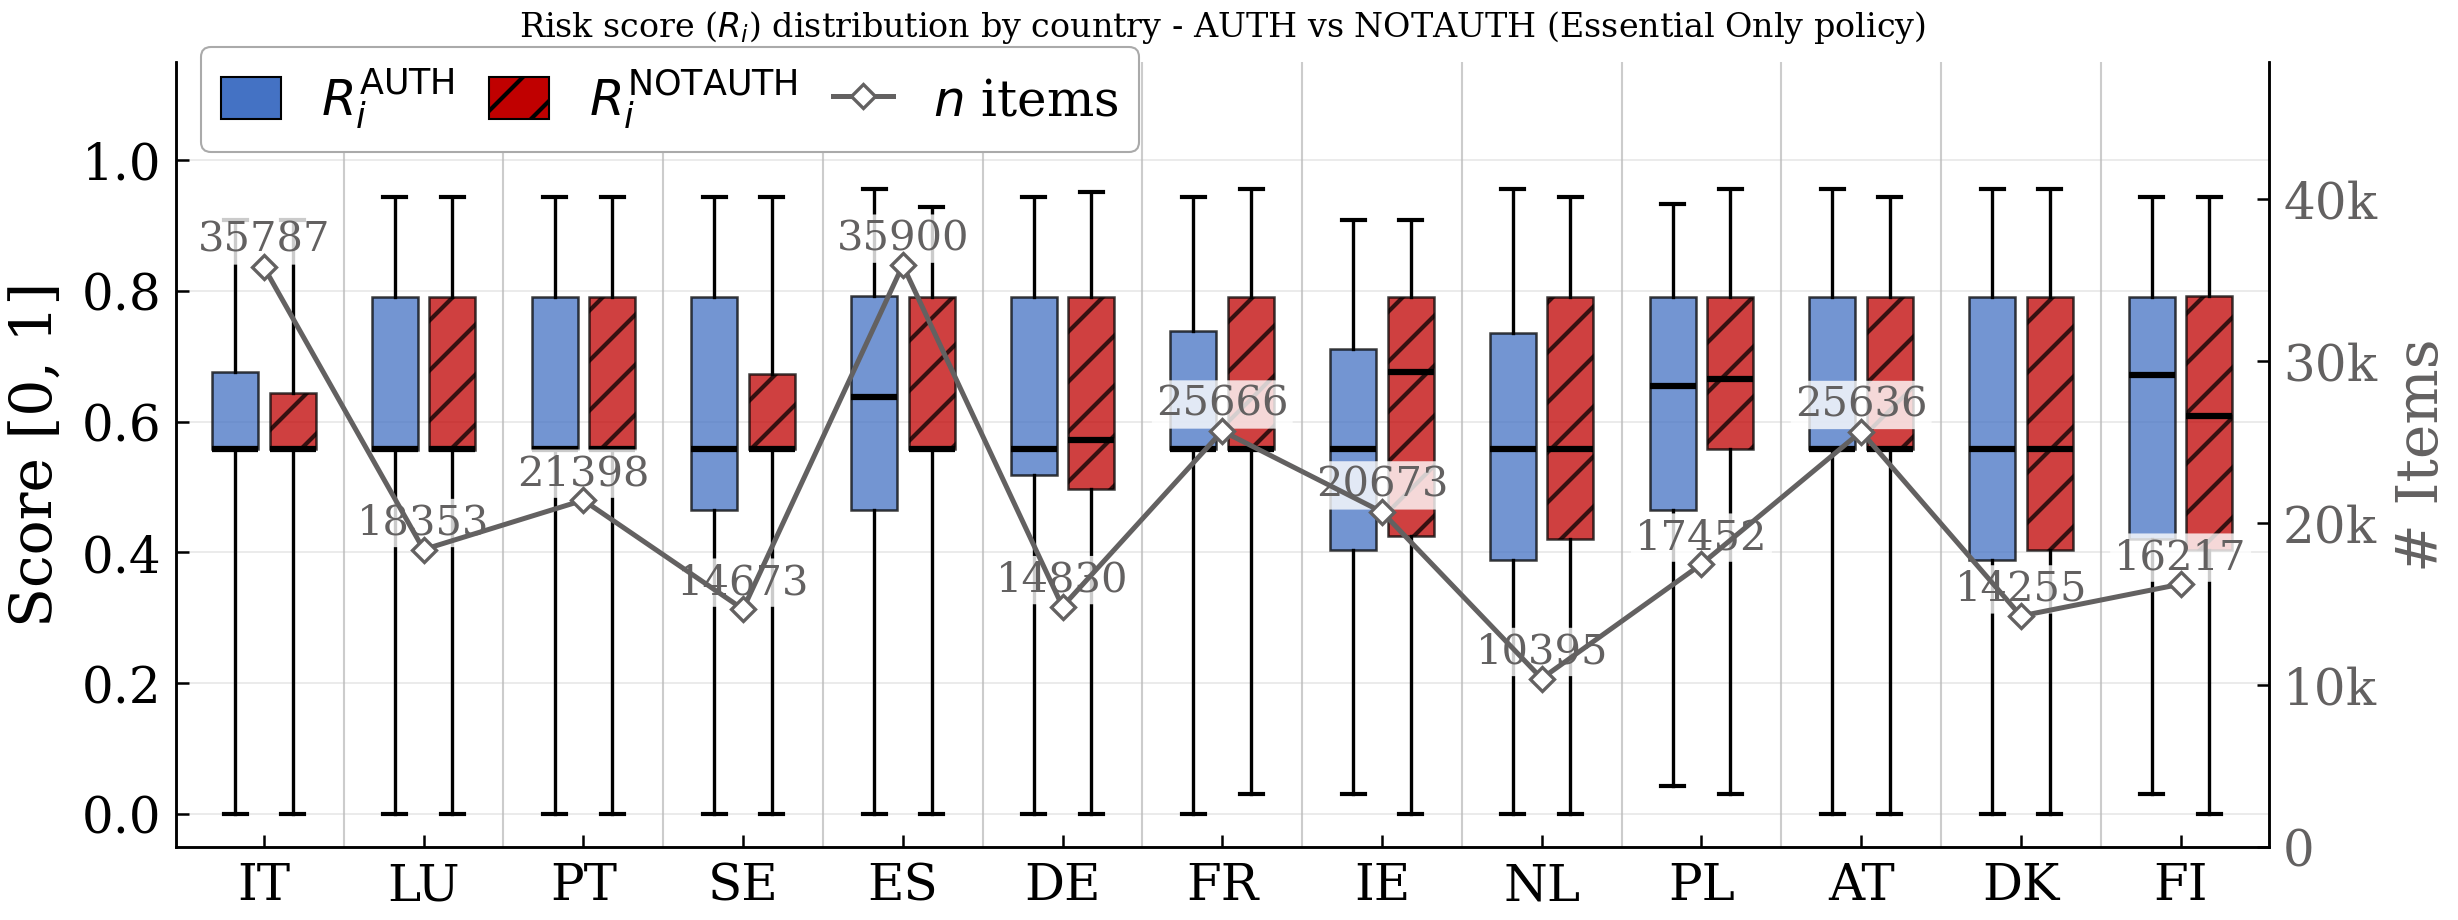
\includegraphics[width=0.92\textwidth]{risk_analysis_PxI_countries/src/outputs/figures/f2_risk_by_country_and_mode.png}
\caption{Risk score ($R_i$) distribution across the thirteen countries, AUTH vs
NOTAUTH, all storage types pooled, Essential Only (\code{PARTIAL}) policy. Line
overlay is item count per country.}
\label{fig:f2}
\end{figure}

\begin{figure}[h]
\centering
\begin{subfigure}{0.48\textwidth}
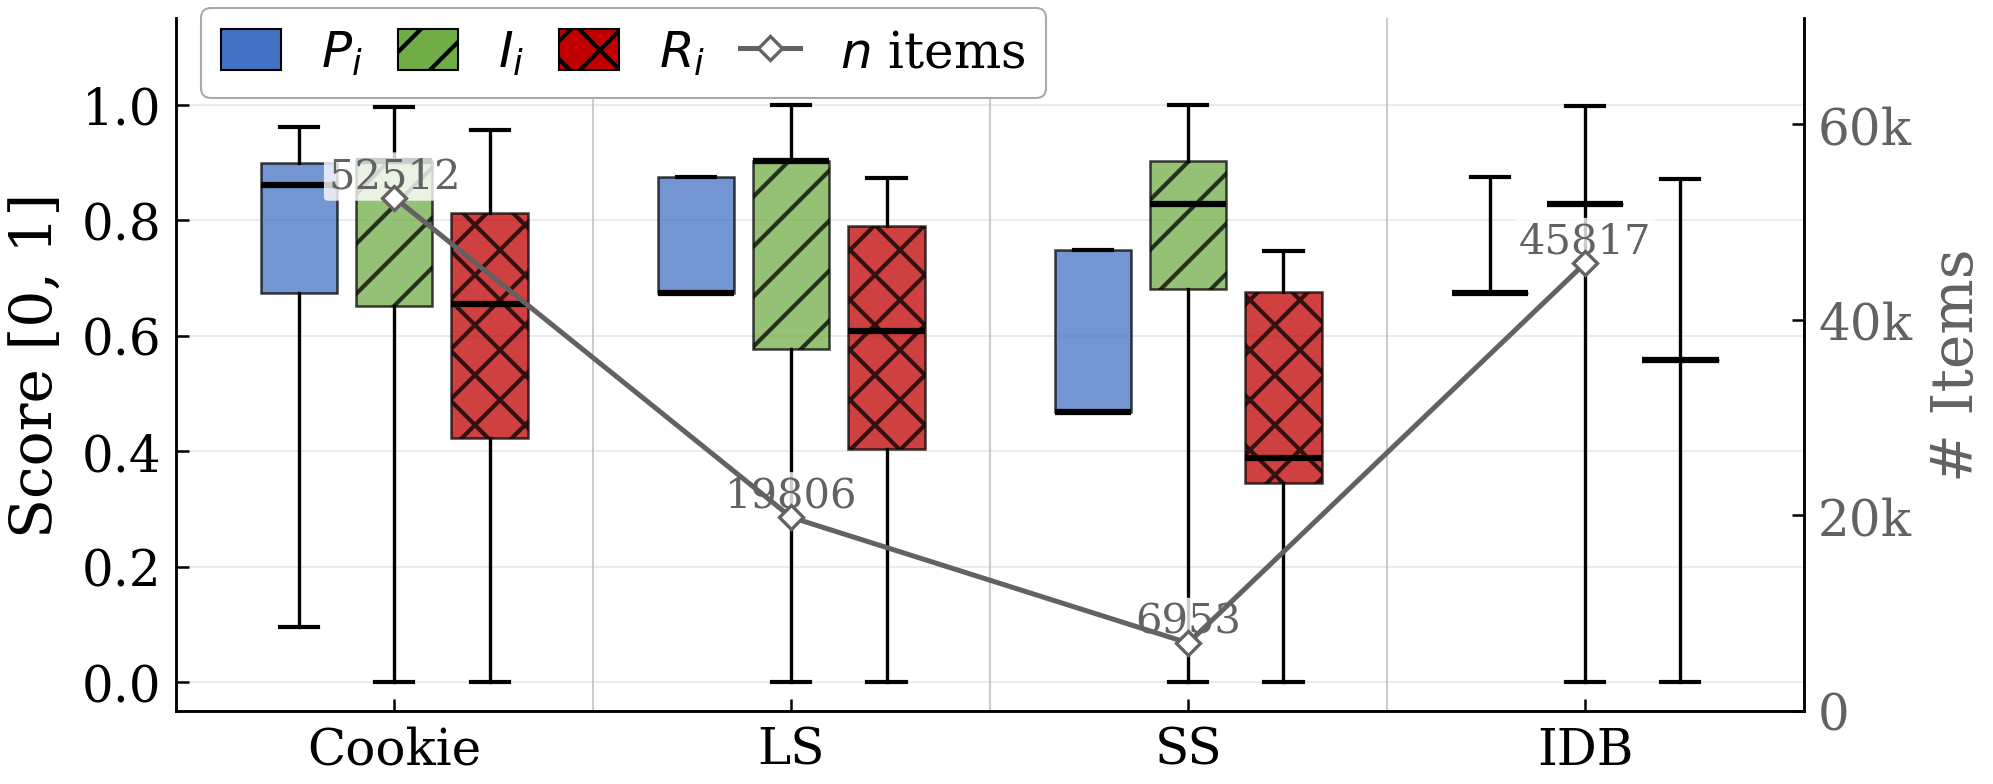
\includegraphics[width=\textwidth]{risk_analysis_PxI_countries/src/outputs/figures/f1_metrics_by_storage_AUTH_all_PARTIAL.png}
\caption{AUTH, all countries pooled}
\end{subfigure}
\hfill
\begin{subfigure}{0.48\textwidth}
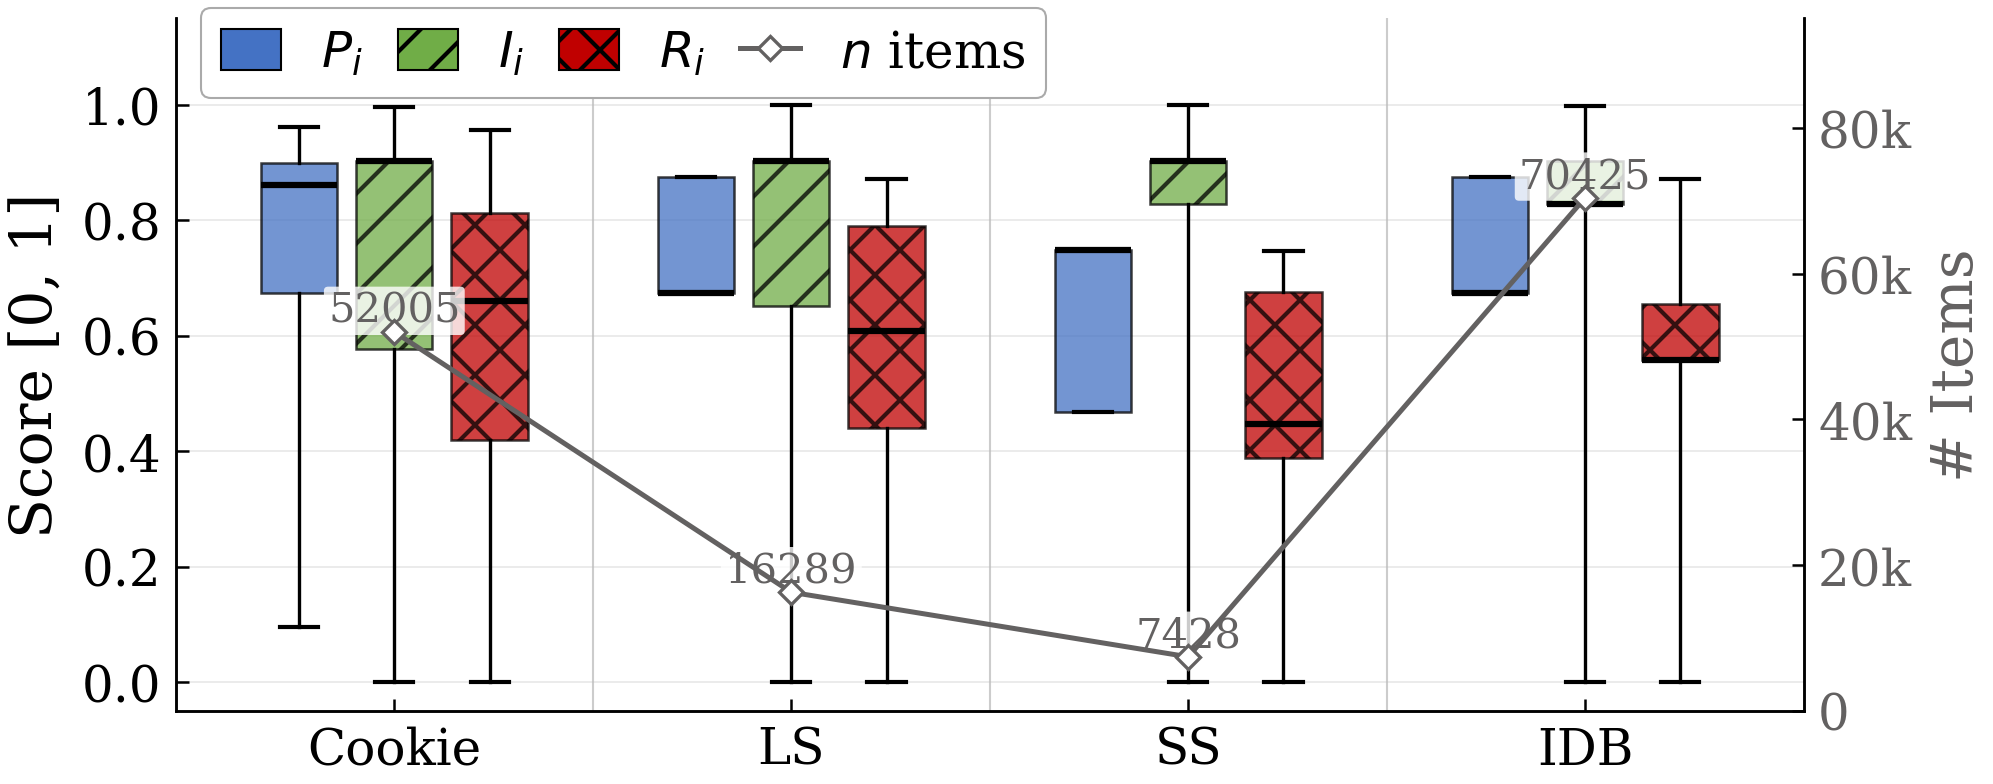
\includegraphics[width=\textwidth]{risk_analysis_PxI_countries/src/outputs/figures/f1_metrics_by_storage_NOTAUTH_all_PARTIAL.png}
\caption{NOTAUTH, all countries pooled}
\end{subfigure}
\caption{Exposure ($P_i$), impact ($I_i$), and risk ($R_i$) distributions by storage type, pooled across all thirteen countries.}
\label{fig:f1_pooled}
\end{figure}

Per-country versions of Figure~\ref{fig:f1_pooled} (26 figures, one per
country/mode combination) are provided in Appendix~\ref{app:f1}.

% ============================================================
\section{Discussion and Limitations}
\label{sec:limitations}
% ============================================================

This section states plainly what can and cannot be concluded from the
numbers above.

\subsection{What is solid}

The literal \code{DIRECT\_PII} matches (email, phone, name, address, date of
birth) are matched against exact strings known from each synthetic persona --
there is no ambiguity and no false-positive risk for these specific fields.
This is the one part of the pipeline with genuine ground truth.

\subsection{Categorization-layer caveats}

\begin{itemize}[leftmargin=1.3cm]
  \item A regex bug that matched long digit chains (e.g. TCF consent
    strings) as IP addresses was found and fixed for the country pipeline
    only; whether the original FR pipeline carries the same bug was out of
    scope and was not checked.
  \item A duplication bug in cookie categorization caused some
    subcategories (e.g. \code{gender}) to be counted up to $\sim$29$\times$
    per real occurrence; fixed for the country pipeline. Its status in the
    FR pipeline is likewise unverified.
  \item \code{DIRECT\_PII\_KEYS}'s \code{user\_id\_key} pattern is known to
    be dominated by non-PII matches (consent-platform tokens, generic
    numeric session IDs, the literal string \code{"anonymous"}) -- this was
    identified but left unfixed by explicit decision.
  \item The first LLM categorization pass batches \code{IndexedDB} records by
    record count rather than field count, so records with 50+ uncategorized
    fields could silently exceed the model's output limit and lose fields
    with no error raised. A dedicated field-capped correction pass was added
    specifically to recover these; because that correction pass has since
    run (and itself mutated the UNCATEGORIZED file in place), the original
    truncation rate can no longer be reconstructed precisely from the current
    data for all thirteen countries -- it is a documented mechanism, not a
    number this revision can still quote.
\end{itemize}

\subsection{Risk-model caveats}

\begin{itemize}[leftmargin=1.3cm]
  \item Both the exposure coefficients and the impact map are fixed expert
    judgments, not values fit to observed outcomes. They provide a
    consistent \emph{relative} ranking under one set of assumptions, not a
    validated absolute probability of harm.
  \item \textbf{No sensitivity analysis has been run on these weights for
    the country dataset} (explicitly deferred). Country rankings by risk
    should be treated as conditional on this one weight set until that
    analysis is done.
  \item For \code{localStorage}, \code{sessionStorage}, and
    \code{IndexedDB}, the exposure features (\code{js\_accessible},
    \code{network\_exposed}, \code{cross\_site}, \code{persistent}) are
    hardcoded constants per storage type rather than measured per item --
    only the third-party flag varies. $P_i$, and hence $R_i$, is therefore
    close to a two-valued step function for these three storage types,
    which is why Table~\ref{tab:risk_by_storage_auth} looks largely uniform
    across countries. Only cookies carry a genuinely continuous exposure
    score in the current model.
  \item The impact engine computes an entropy/structuredness ``boost'' that
    is never applied (the multiplication is commented out in the ported
    source) -- highly unique or structured values currently receive no
    impact premium despite the formula suggesting they should.
  \item $R_i = P_i \times I_i$ assumes exposure and impact are independent,
    which is a simplification.
\end{itemize}

\subsection{Cross-country comparison caveats}

\begin{itemize}[leftmargin=1.3cm]
  \item Each persona completed \emph{one} crawl session on
    country-appropriate sites; site selection was not held constant across
    countries. A volume or category difference between two countries may
    reflect genuinely different tracking practices, or simply which sites
    (a game portal vs.\ a grocery site) that persona happened to visit --
    \code{IT\_0573}'s outsized \code{DEVICE\_ENV} and \code{IndexedDB}
    volumes, and \code{FR\_0429}'s extreme NOTAUTH/AUTH ratio, are
    plausible instances of this.
  \item With one crawl per persona per authentication mode, there is no
    way to distinguish a stable population-level difference from that
    single run's noise. No confidence intervals or significance tests are
    computed anywhere in this pipeline -- every figure above is a
    descriptive statistic, not an inferential one. With thirteen personas
    instead of six, the spread of per-country ratios and shares is wider
    than it first appeared, not narrower -- a reminder that adding more
    single-session personas increases the \emph{range} of outcomes observed
    without adding any statistical power to generalize from it.
  \item Third-party detection is a simple domain-suffix check and does not
    catch more advanced first-party-disguise techniques (e.g.\ CNAME
    cloaking); the vendor name list is a static, incomplete hand-authored
    mapping, so an unrecognized ``top vendor'' (e.g.\ \code{a-mo.net} for
    \code{ES\_0290}) may just mean \emph{unclassified domain}, not
    \emph{identified major tracker}.
  \item Cookie lifetime/duration figures computed via the lifecycle
    analysis script are not exactly reproducible across reruns, because
    that script measures duration against the time the script is run
    rather than the time of data collection -- a pre-existing quirk
    inherited from the FR codebase. This report does not use that script's
    output.
\end{itemize}

% ============================================================
\section{Conclusion}
% ============================================================

Across the thirteen country personas, tracking-oriented \code{BEHAVIORAL\_DATA}
remains the single largest category overall and leads in ten of the thirteen
countries, but \code{IDENTITY\_TRACKING} leads in \code{IE\_0504} and
\code{DK\_0199}, and \code{ID\_SOLUTIONS\_AND\_EXCHANGES} leads in
\code{FI\_0373} -- the ``\code{BEHAVIORAL\_DATA} everywhere'' pattern visible in
the earlier six-country sample does not hold once more countries are added.
\code{IndexedDB} is the largest storage type in most, but not all, countries
(35.1\%--89.6\% of items). Authentication status still shifts
volume on average -- NOTAUTH collects 1.30$\times$ as many
categorized items as AUTH, pooled -- but that pattern now reverses for three
of the thirteen countries (IE\_0504, AT\_0077, FI\_0373), which the six-country sample had
no opportunity to reveal. Cookie security is weak everywhere: only about a
quarter of cookies in any country are fully conformant (\code{httpOnly} and
\code{secure} together), and no country is uniformly best or worst across the
security attributes examined.

At the risk-score level, per-item severity remains broadly comparable across
countries -- Figure~\ref{fig:f2} shows overlapping distributions and similar
means (0.5894 AUTH vs.\ 0.5945 NOTAUTH, pooled) -- so the
country-to-country differences visible in the raw data are driven far more by
\emph{volume} (how much was collected, which now varies by a factor of
6.29$\times$) than by \emph{per-item severity} (how bad each item
is). This conclusion is now observed over more than twice as many personas as
the original six-country report and still holds, which is some evidence it is
not an artifact of the first six personas chosen -- but it is also a direct
consequence of the current exposure model's structural limitation for
non-cookie storage, and should be revisited once a richer per-item exposure
model and a formal sensitivity analysis are in place. Both are natural next
steps for this line of work, as is adding a second crawl per persona to
separate genuine country-level signal from single-session noise -- a gap this
revision's wider, more erratic ratios and shares has made more visible, not
less.

\appendix

% ============================================================
\section{Per-Country Risk Distribution Figures}
\label{app:f1}
% ============================================================

\begin{figure}[h]
\centering
\begin{subfigure}{0.48\textwidth}
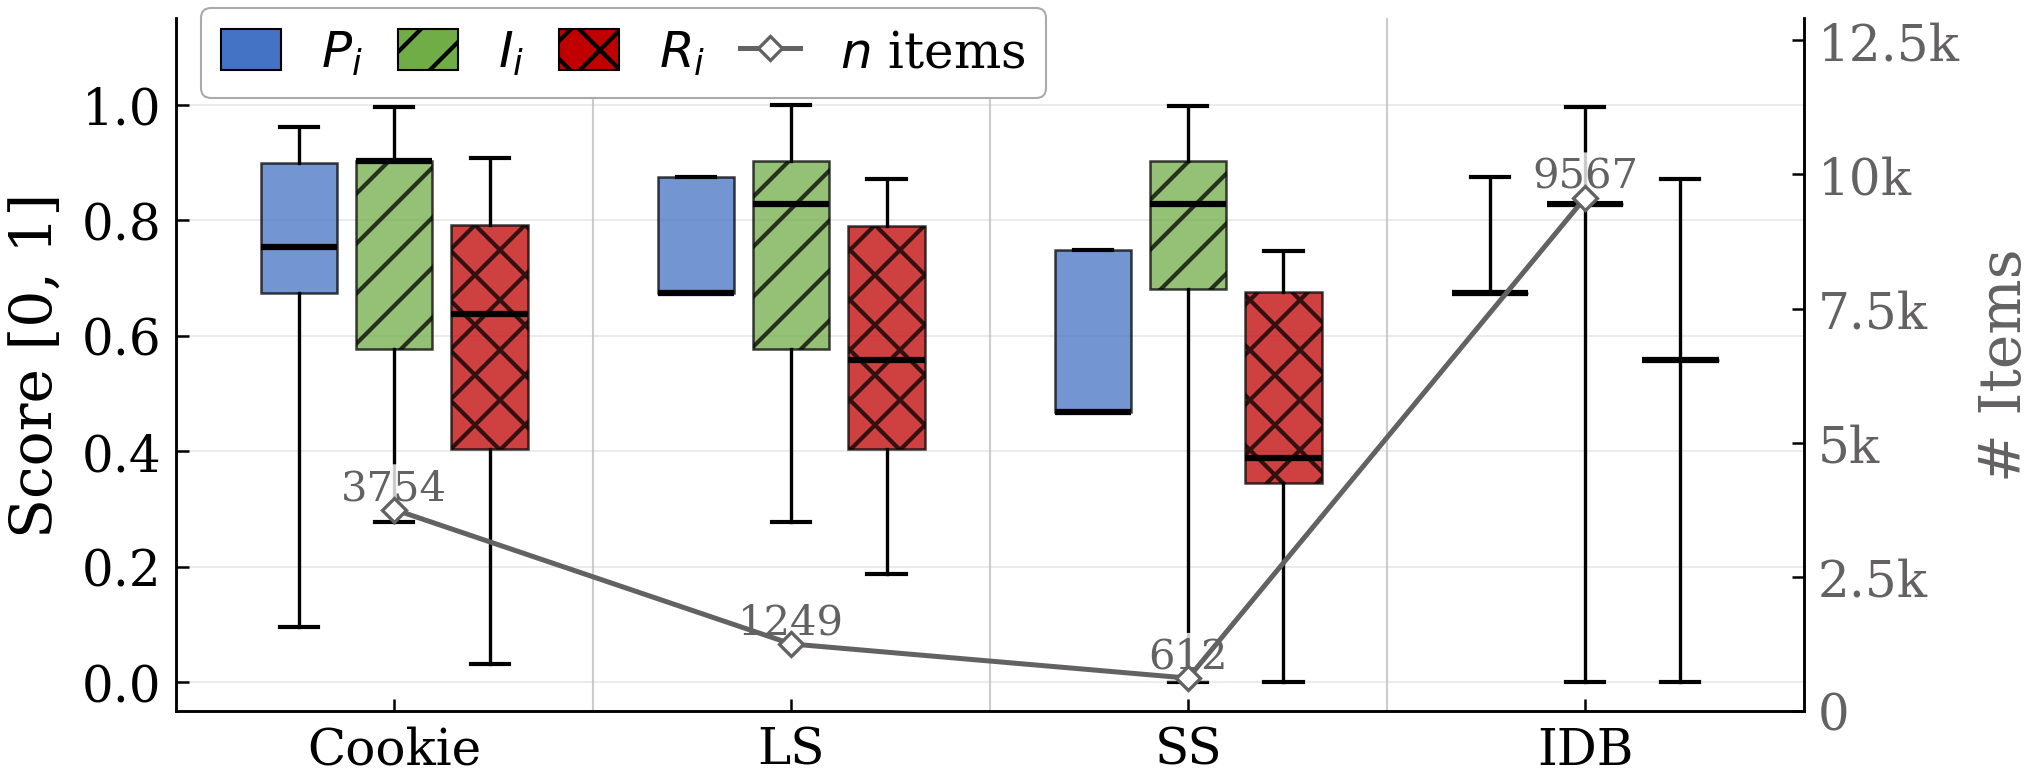
\includegraphics[width=\textwidth]{risk_analysis_PxI_countries/src/outputs/figures/f1_metrics_by_storage_AUTH_IT_0573_PARTIAL.png}
\caption{IT\_0573 -- AUTH}
\end{subfigure}\hfill
\begin{subfigure}{0.48\textwidth}
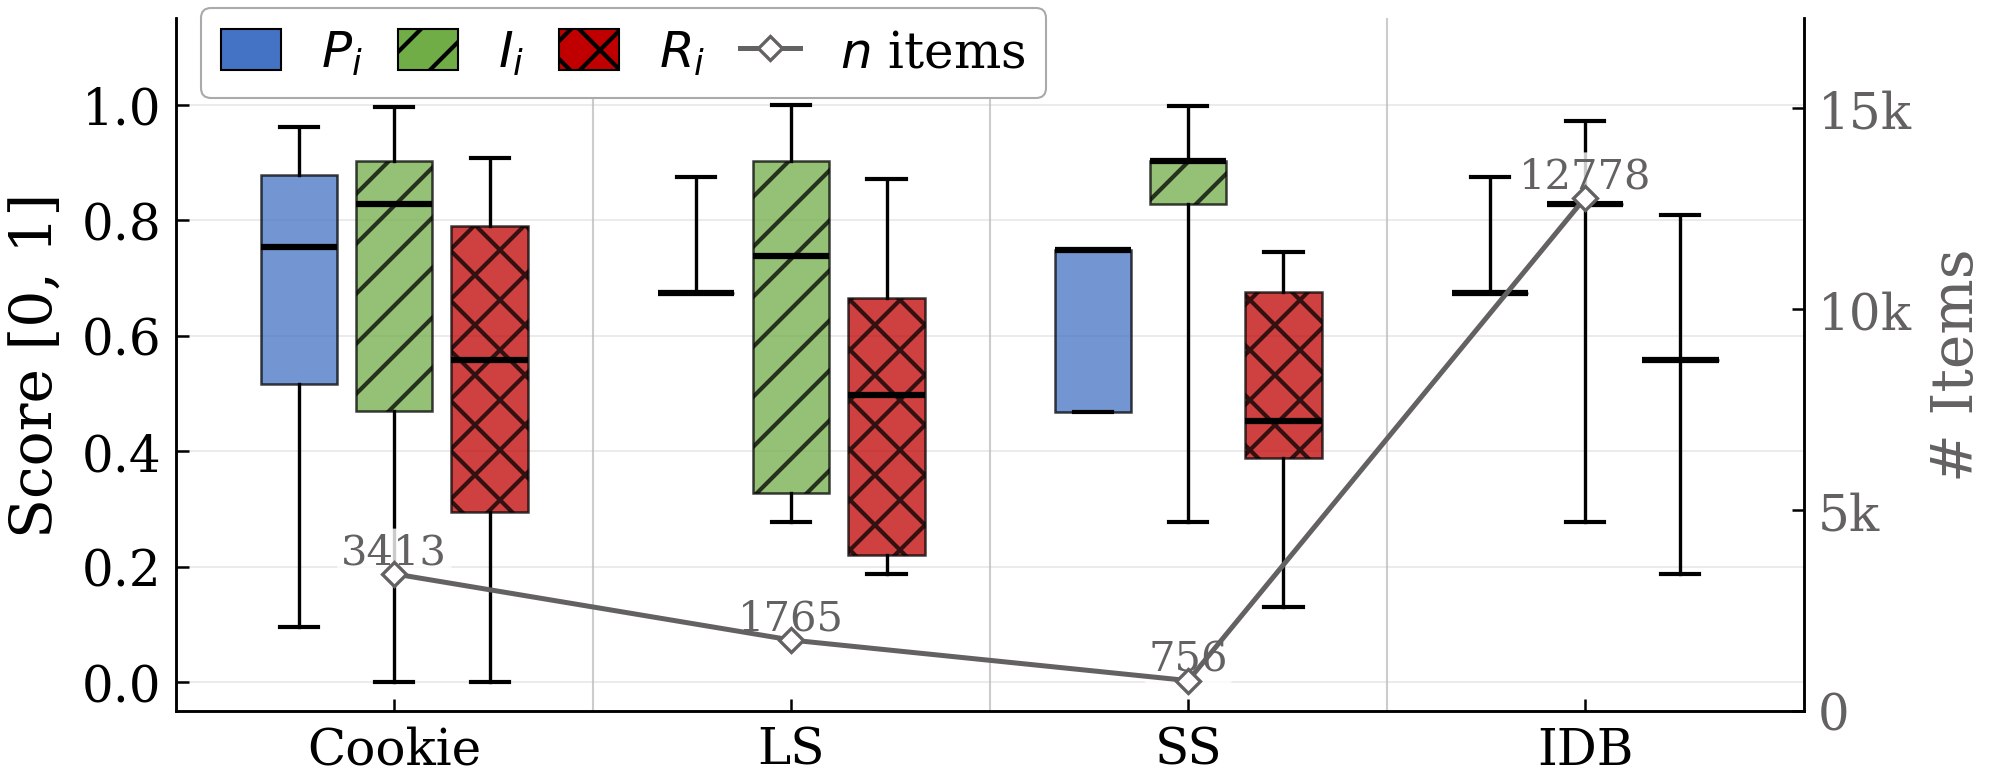
\includegraphics[width=\textwidth]{risk_analysis_PxI_countries/src/outputs/figures/f1_metrics_by_storage_NOTAUTH_IT_0573_PARTIAL.png}
\caption{IT\_0573 -- NOTAUTH}
\end{subfigure}
\end{figure}

\begin{figure}[h]
\centering
\begin{subfigure}{0.48\textwidth}
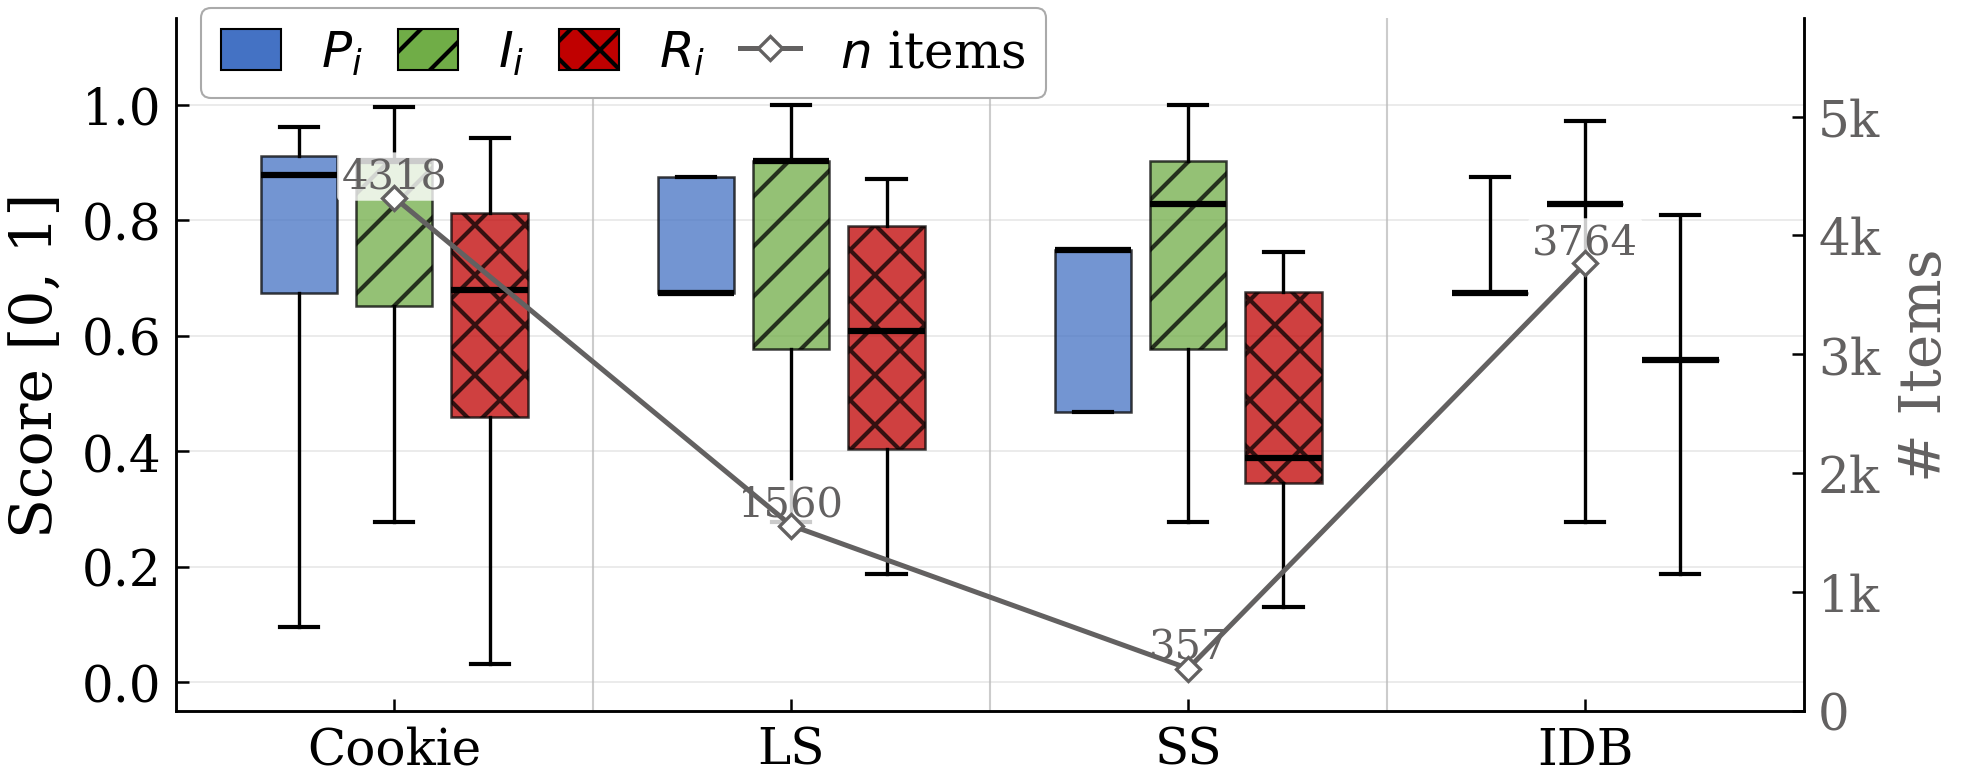
\includegraphics[width=\textwidth]{risk_analysis_PxI_countries/src/outputs/figures/f1_metrics_by_storage_AUTH_LU_0634_PARTIAL.png}
\caption{LU\_0634 -- AUTH}
\end{subfigure}\hfill
\begin{subfigure}{0.48\textwidth}
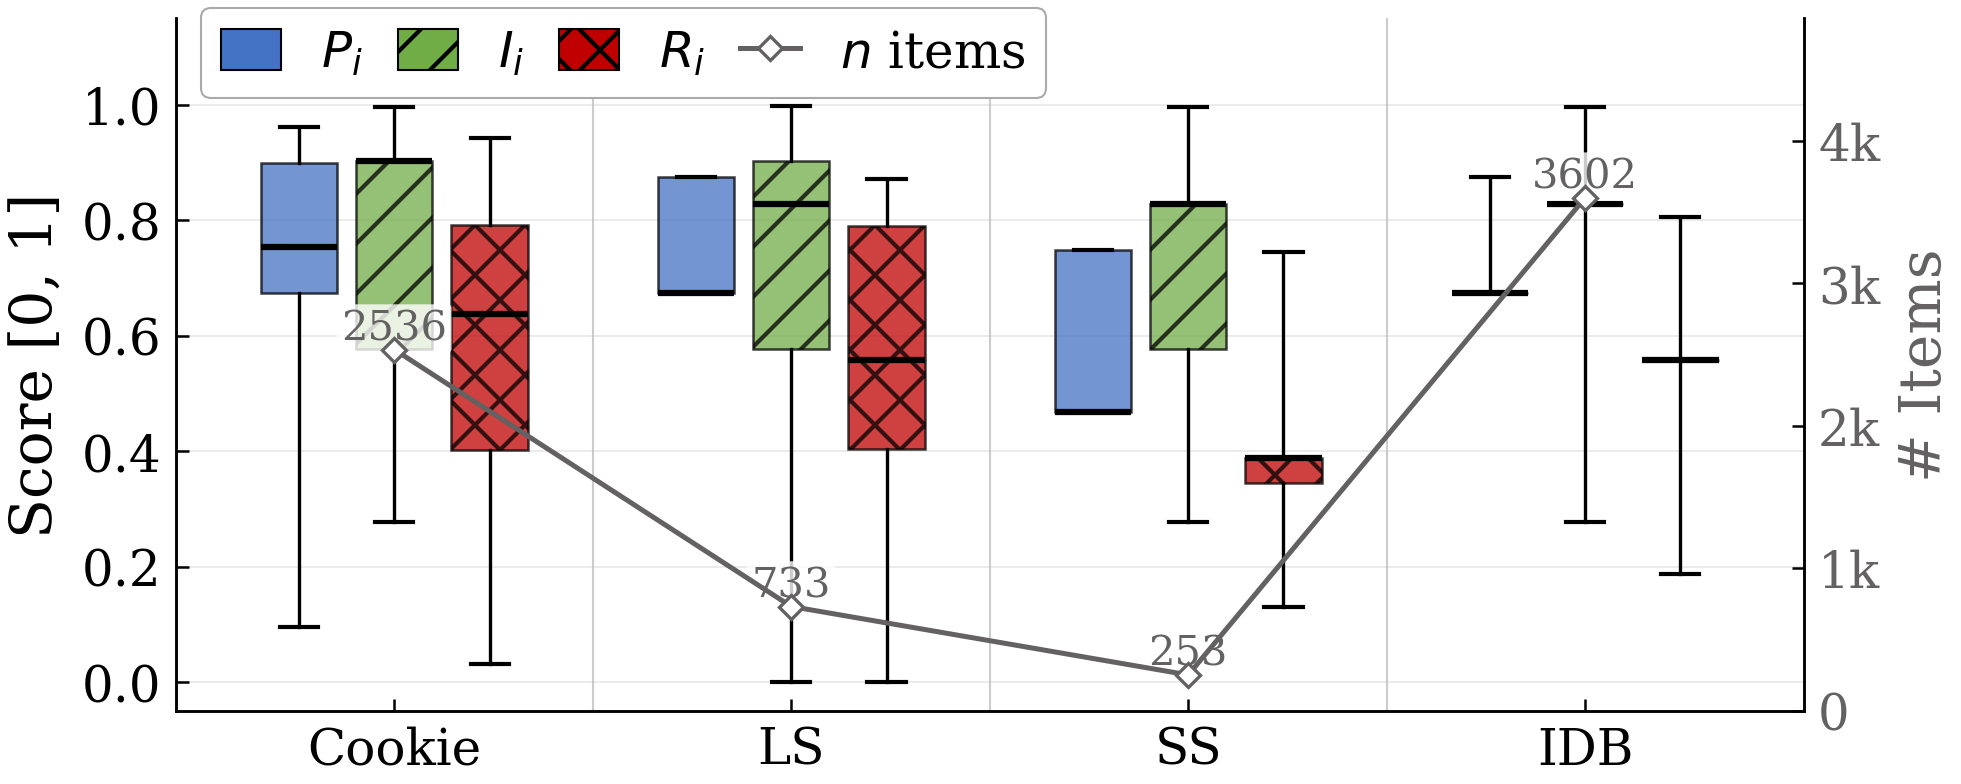
\includegraphics[width=\textwidth]{risk_analysis_PxI_countries/src/outputs/figures/f1_metrics_by_storage_NOTAUTH_LU_0634_PARTIAL.png}
\caption{LU\_0634 -- NOTAUTH}
\end{subfigure}
\end{figure}

\begin{figure}[h]
\centering
\begin{subfigure}{0.48\textwidth}
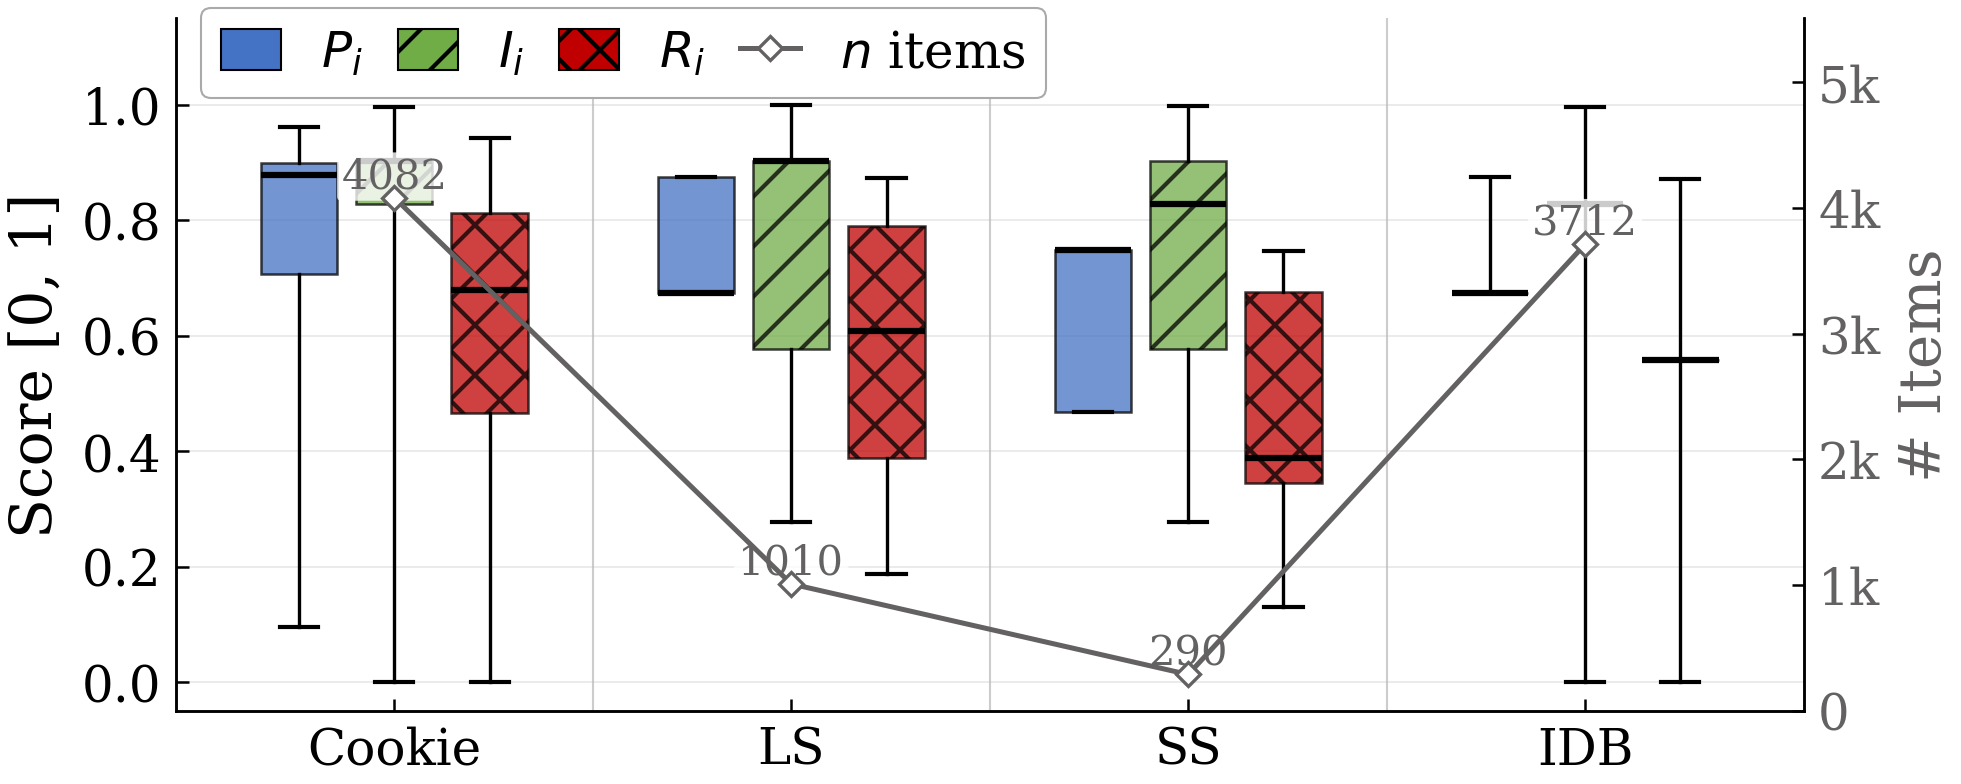
\includegraphics[width=\textwidth]{risk_analysis_PxI_countries/src/outputs/figures/f1_metrics_by_storage_AUTH_PT_0838_PARTIAL.png}
\caption{PT\_0838 -- AUTH}
\end{subfigure}\hfill
\begin{subfigure}{0.48\textwidth}
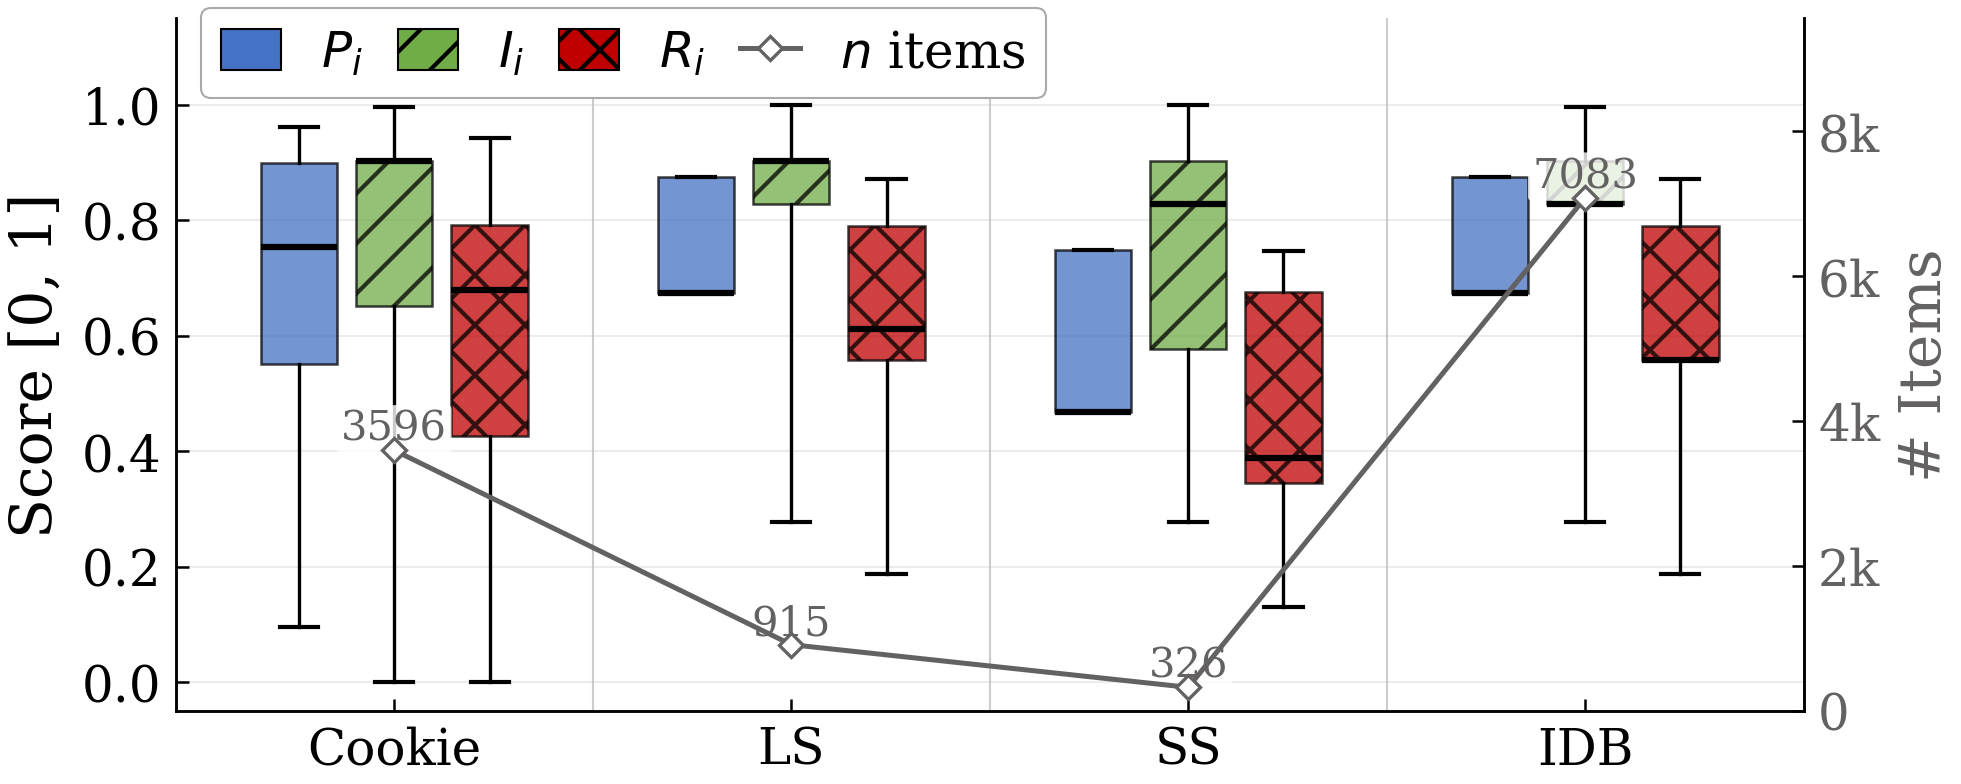
\includegraphics[width=\textwidth]{risk_analysis_PxI_countries/src/outputs/figures/f1_metrics_by_storage_NOTAUTH_PT_0838_PARTIAL.png}
\caption{PT\_0838 -- NOTAUTH}
\end{subfigure}
\end{figure}

\begin{figure}[h]
\centering
\begin{subfigure}{0.48\textwidth}
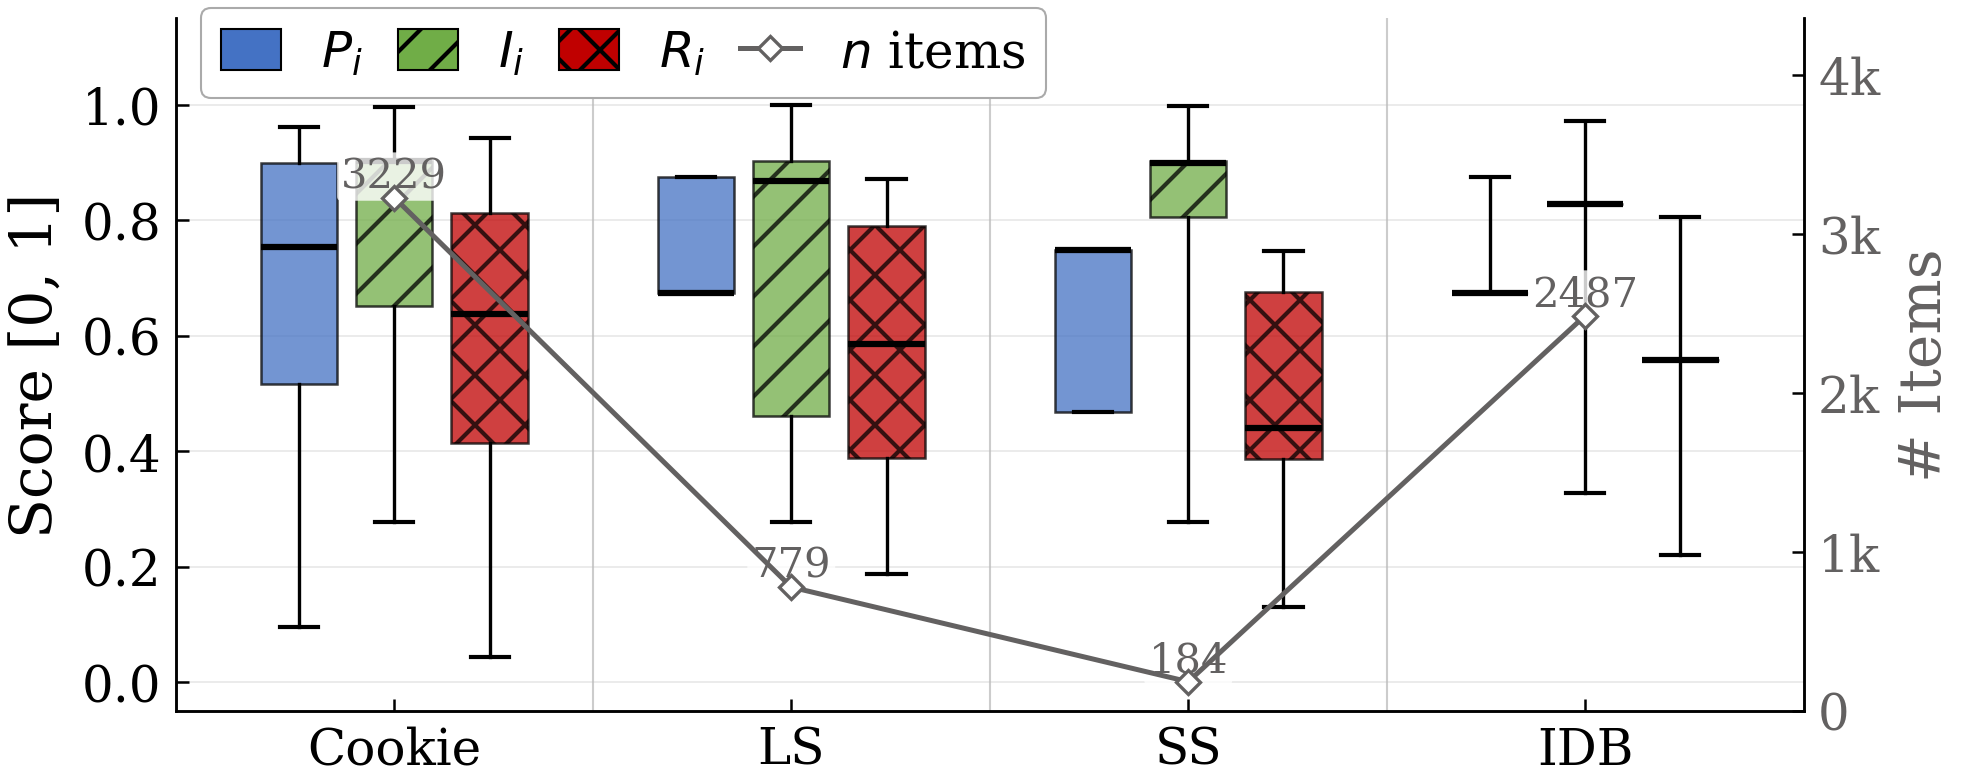
\includegraphics[width=\textwidth]{risk_analysis_PxI_countries/src/outputs/figures/f1_metrics_by_storage_AUTH_SE_0964_PARTIAL.png}
\caption{SE\_0964 -- AUTH}
\end{subfigure}\hfill
\begin{subfigure}{0.48\textwidth}
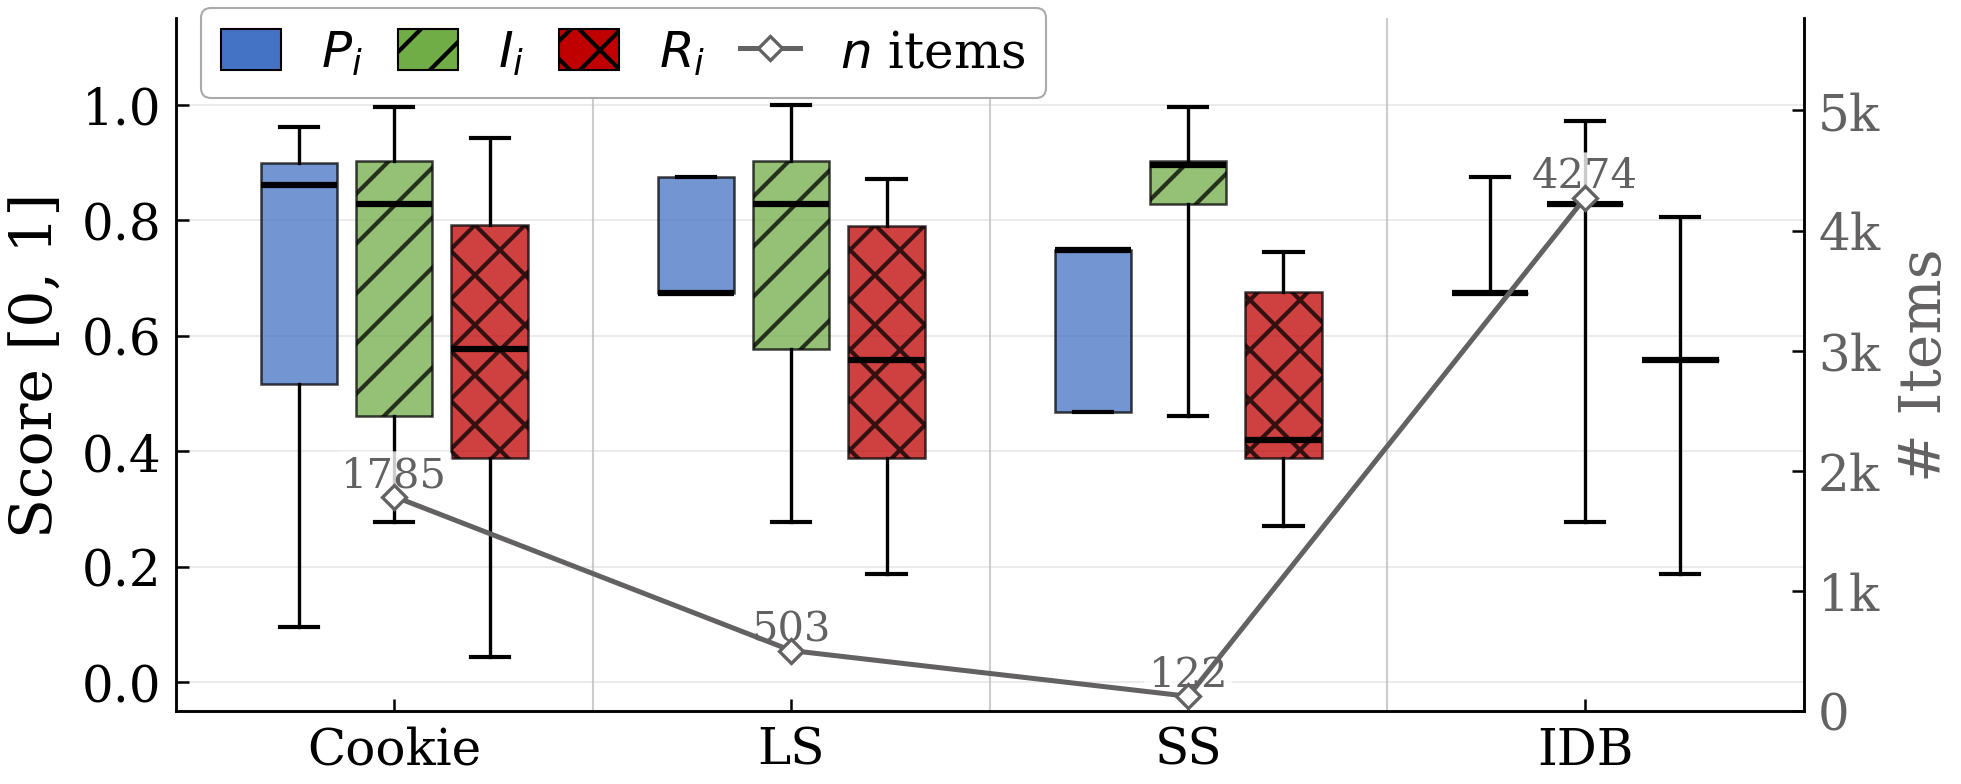
\includegraphics[width=\textwidth]{risk_analysis_PxI_countries/src/outputs/figures/f1_metrics_by_storage_NOTAUTH_SE_0964_PARTIAL.png}
\caption{SE\_0964 -- NOTAUTH}
\end{subfigure}
\end{figure}

\begin{figure}[h]
\centering
\begin{subfigure}{0.48\textwidth}
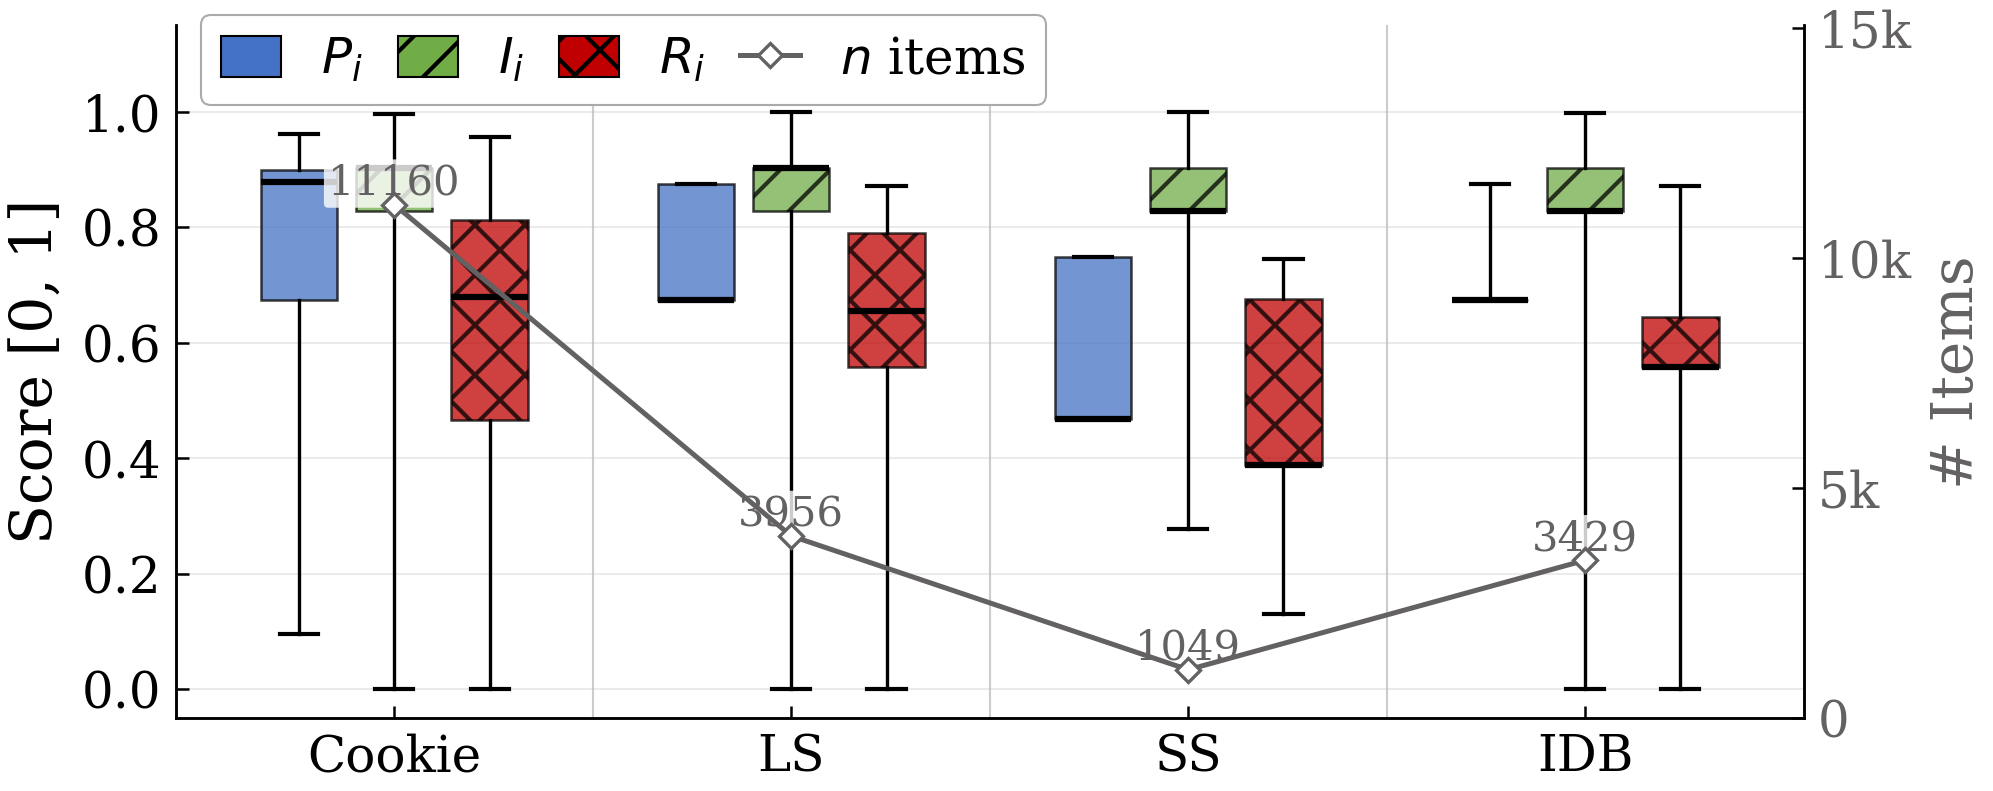
\includegraphics[width=\textwidth]{risk_analysis_PxI_countries/src/outputs/figures/f1_metrics_by_storage_AUTH_ES_0290_PARTIAL.png}
\caption{ES\_0290 -- AUTH}
\end{subfigure}\hfill
\begin{subfigure}{0.48\textwidth}
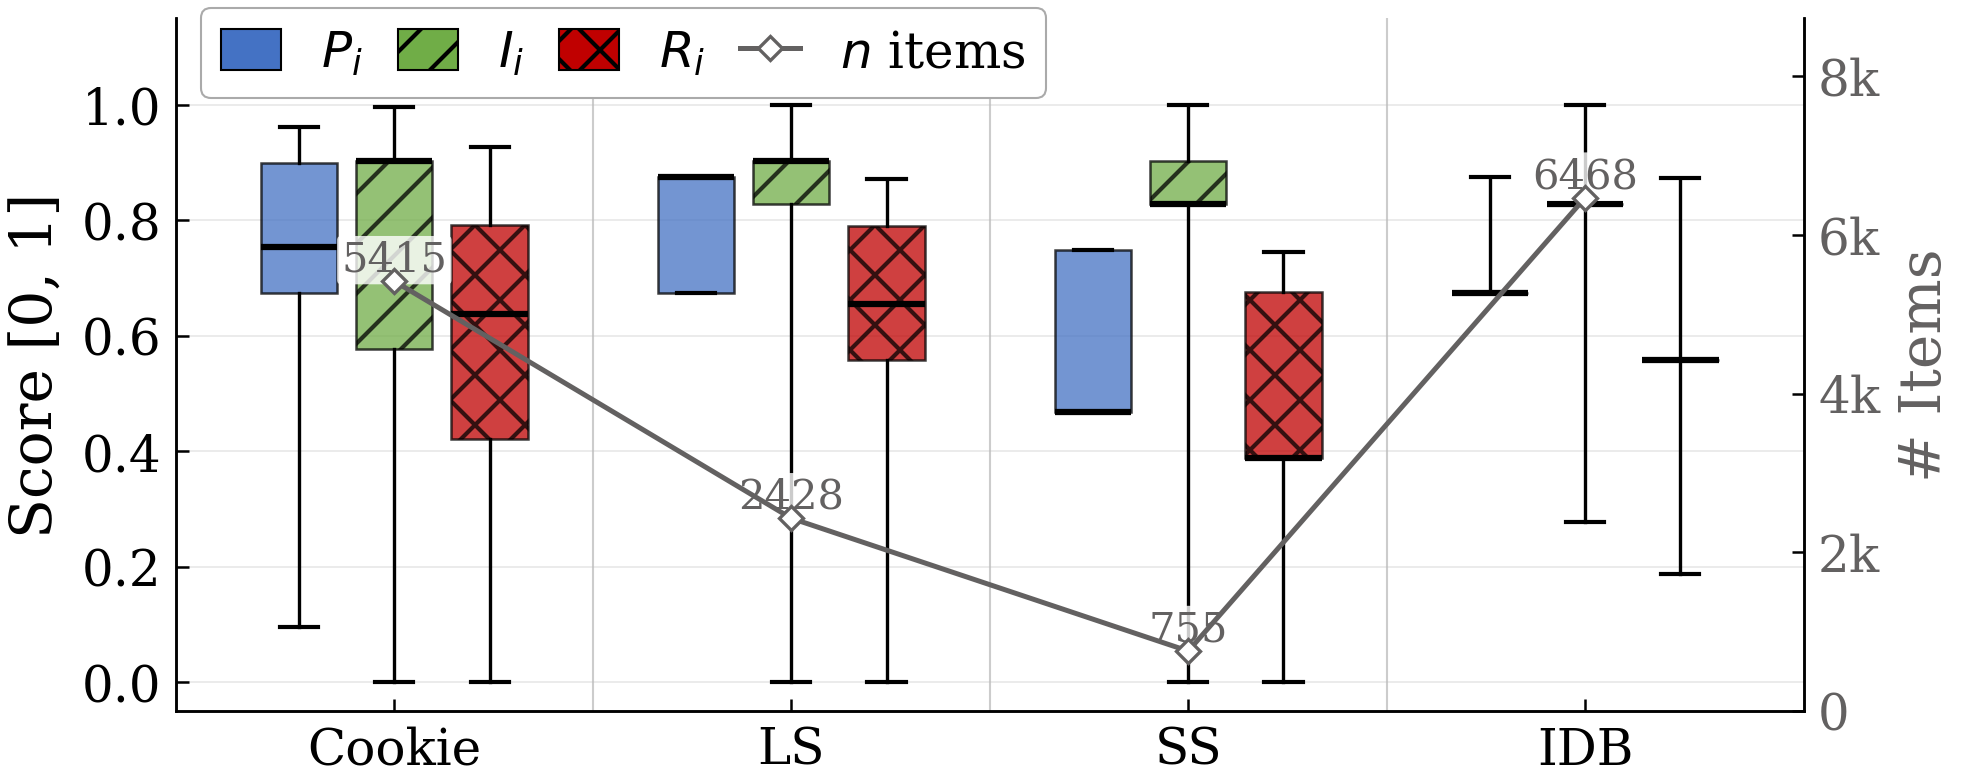
\includegraphics[width=\textwidth]{risk_analysis_PxI_countries/src/outputs/figures/f1_metrics_by_storage_NOTAUTH_ES_0290_PARTIAL.png}
\caption{ES\_0290 -- NOTAUTH}
\end{subfigure}
\end{figure}

\begin{figure}[h]
\centering
\begin{subfigure}{0.48\textwidth}
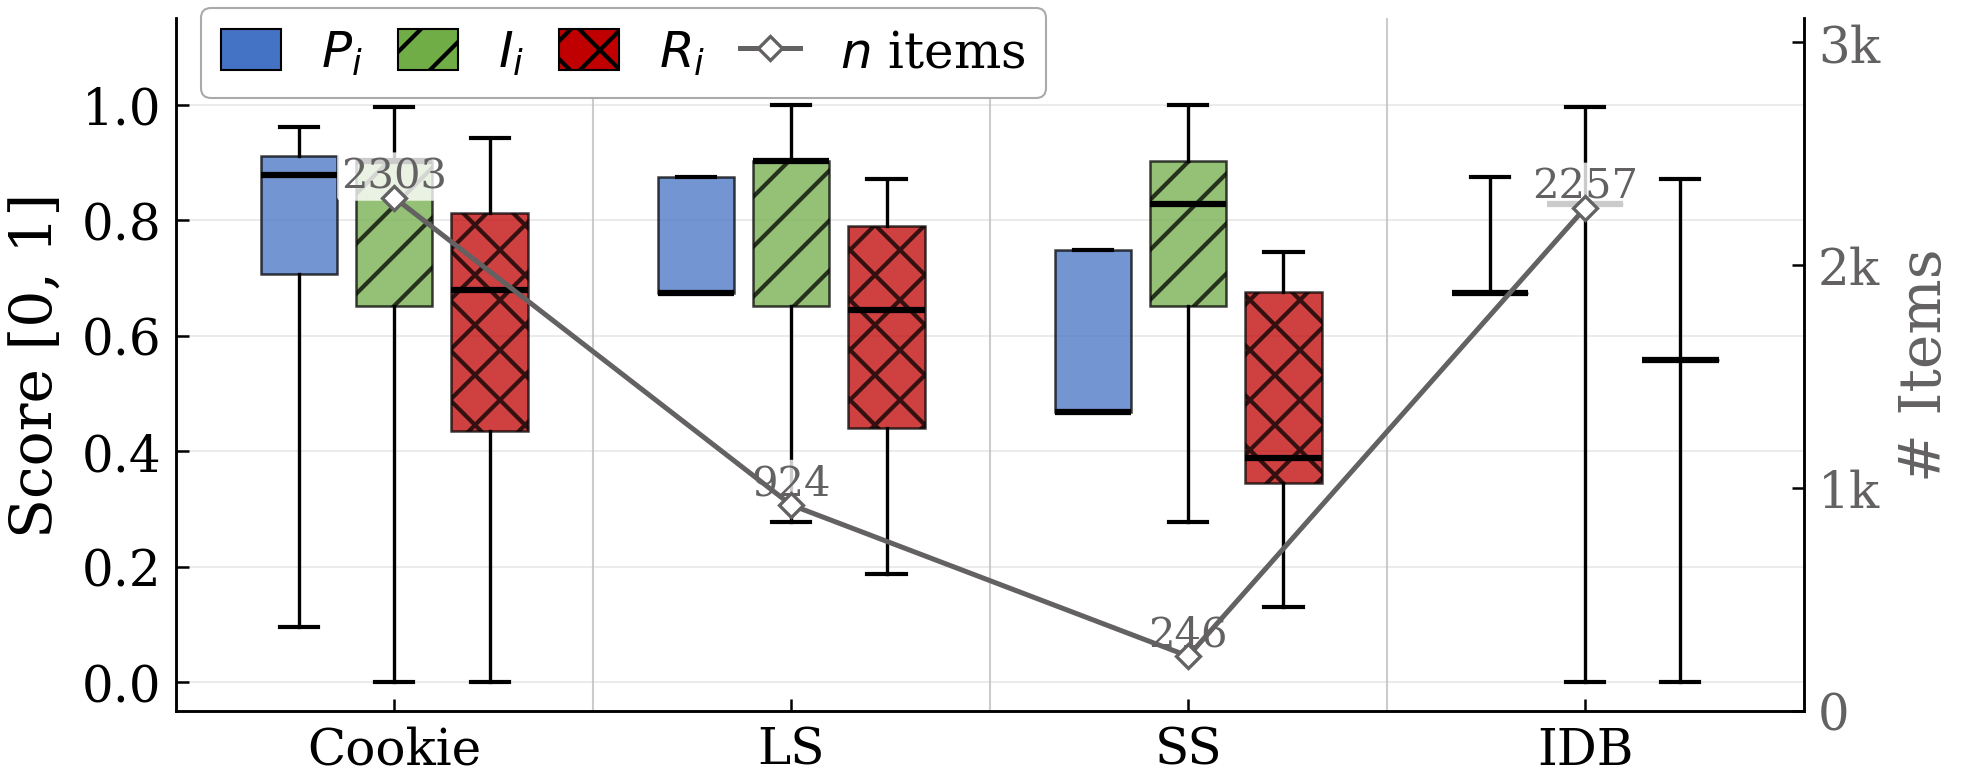
\includegraphics[width=\textwidth]{risk_analysis_PxI_countries/src/outputs/figures/f1_metrics_by_storage_AUTH_DE_0018_PARTIAL.png}
\caption{DE\_0018 -- AUTH}
\end{subfigure}\hfill
\begin{subfigure}{0.48\textwidth}
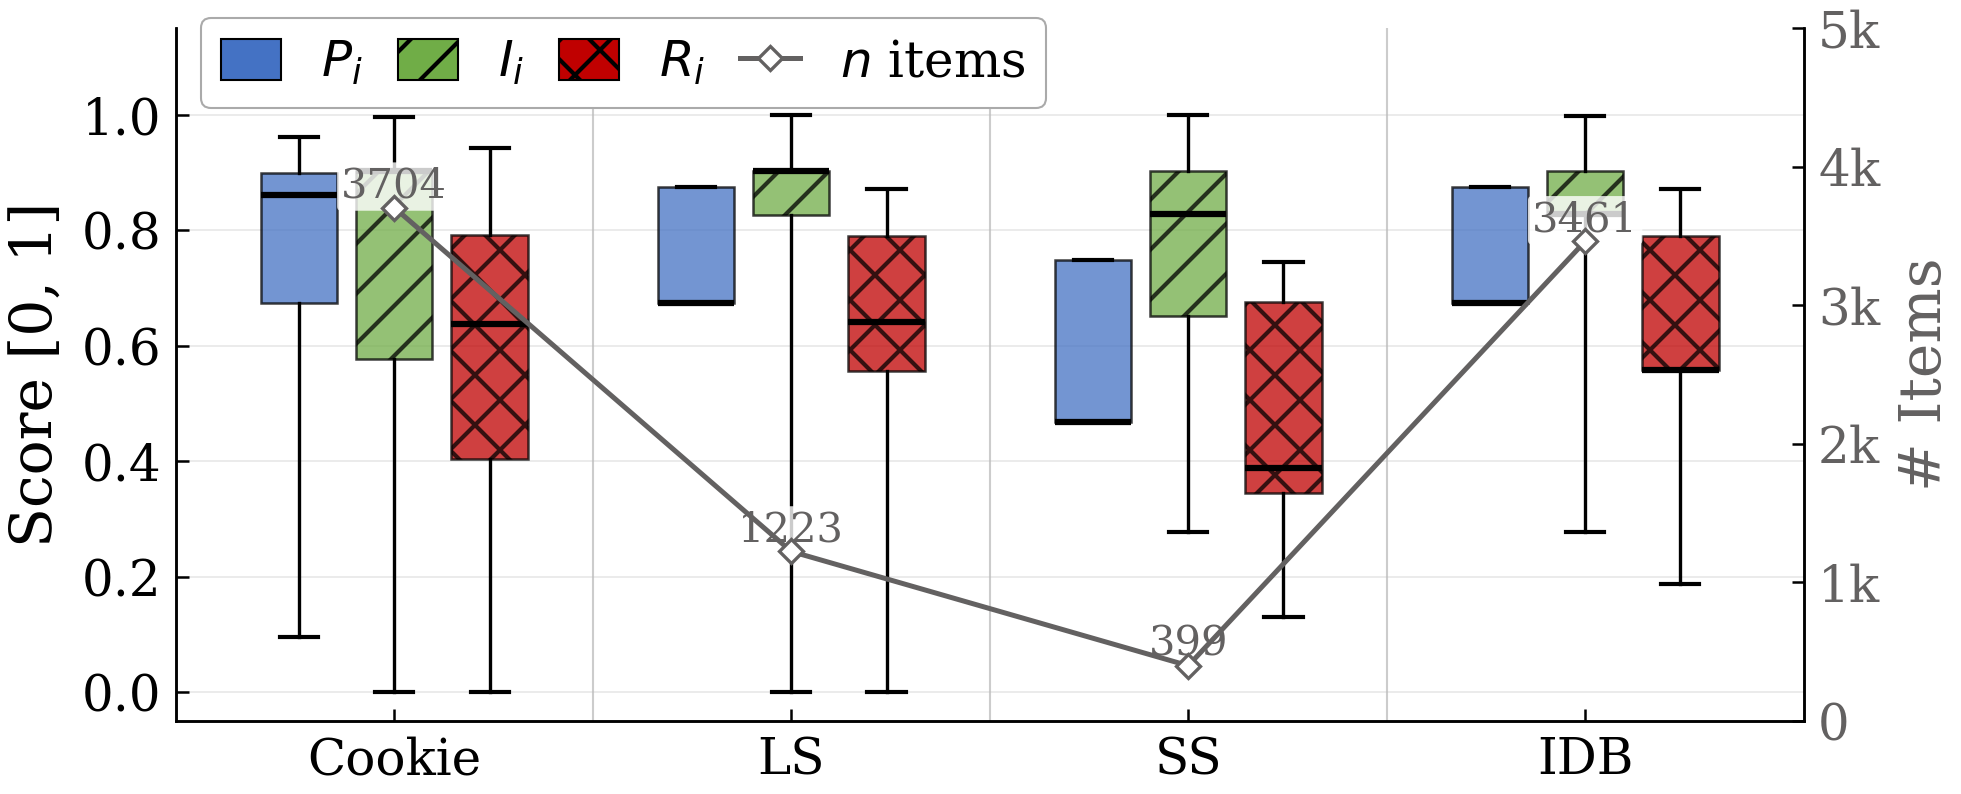
\includegraphics[width=\textwidth]{risk_analysis_PxI_countries/src/outputs/figures/f1_metrics_by_storage_NOTAUTH_DE_0018_PARTIAL.png}
\caption{DE\_0018 -- NOTAUTH}
\end{subfigure}
\end{figure}

\begin{figure}[h]
\centering
\begin{subfigure}{0.48\textwidth}
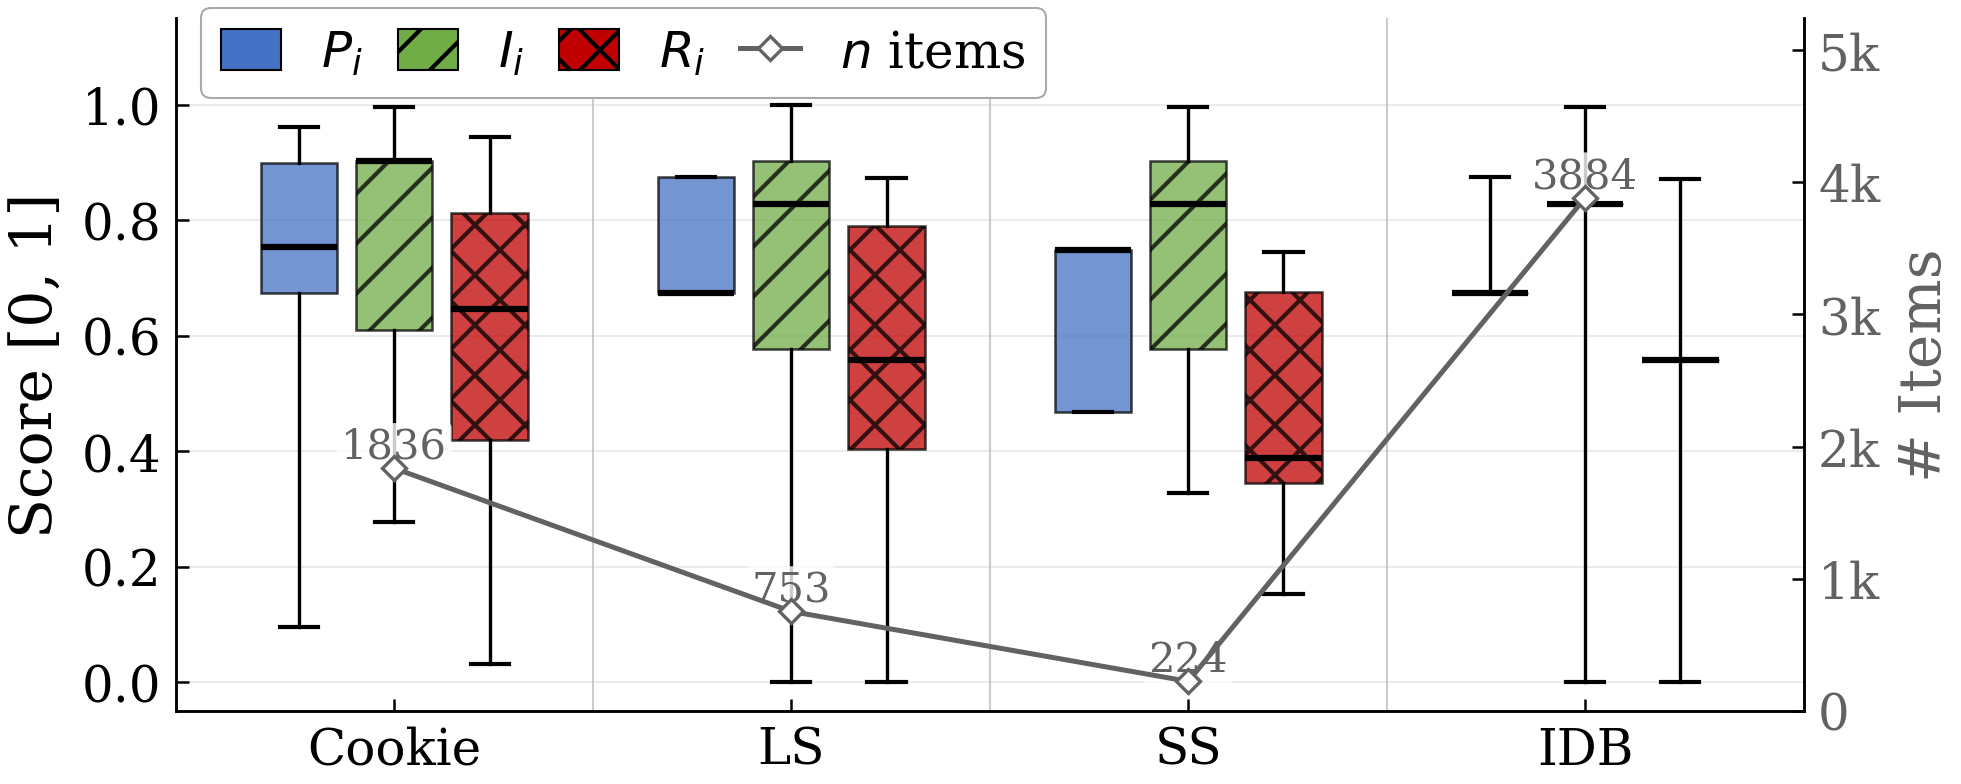
\includegraphics[width=\textwidth]{risk_analysis_PxI_countries/src/outputs/figures/f1_metrics_by_storage_AUTH_FR_0429_PARTIAL.png}
\caption{FR\_0429 -- AUTH}
\end{subfigure}\hfill
\begin{subfigure}{0.48\textwidth}
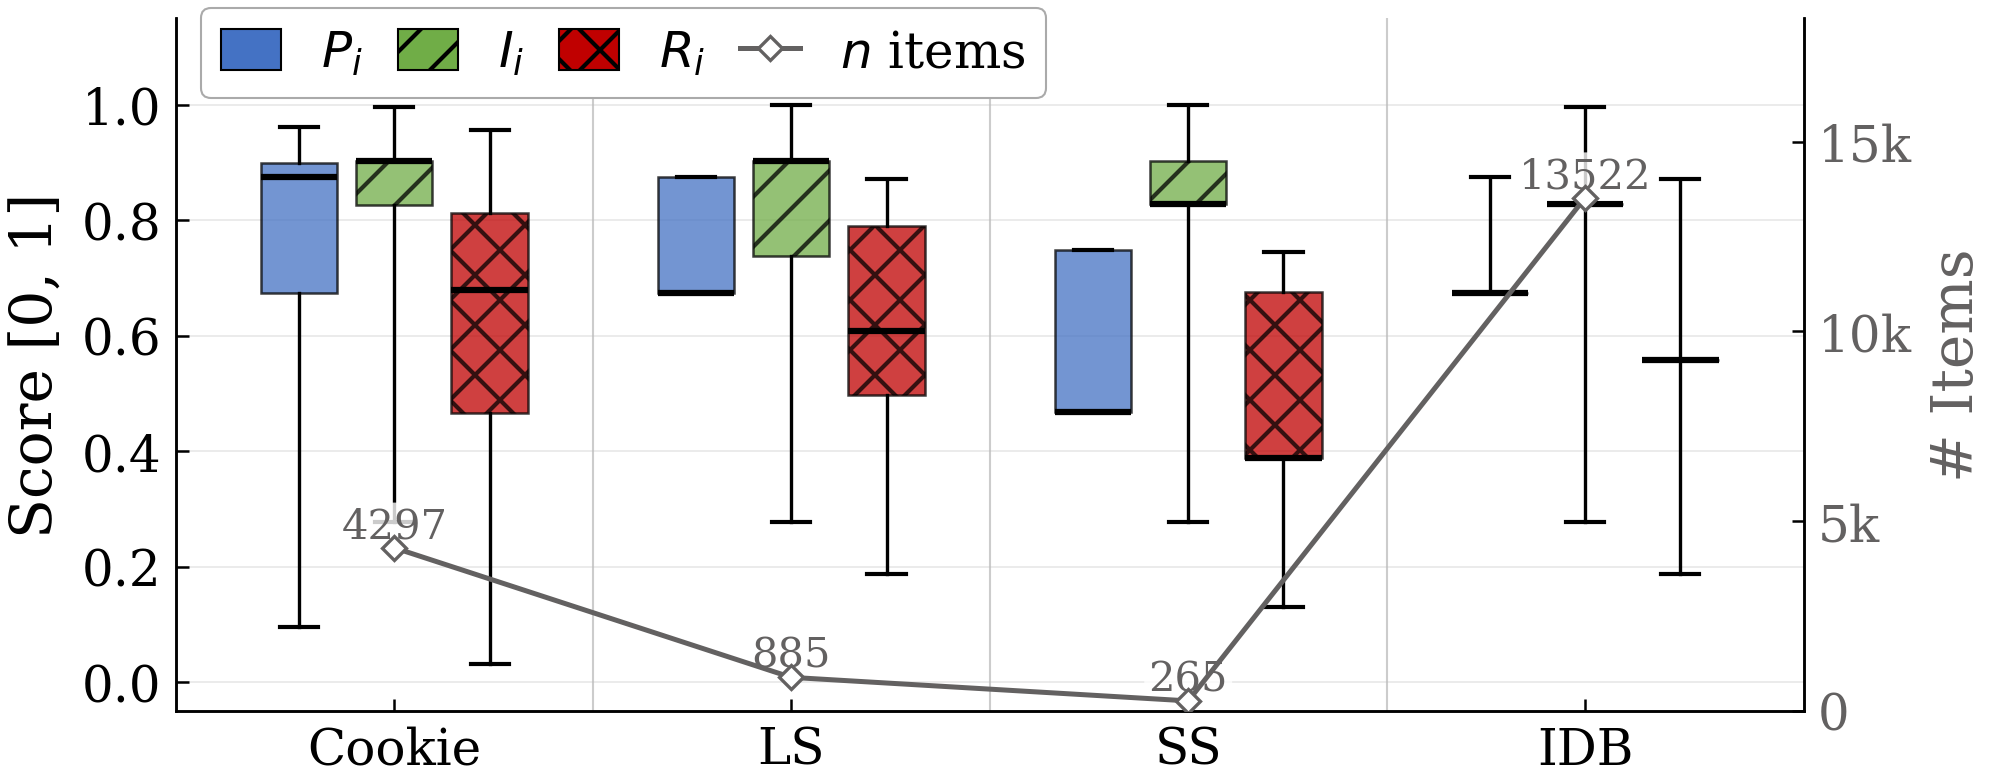
\includegraphics[width=\textwidth]{risk_analysis_PxI_countries/src/outputs/figures/f1_metrics_by_storage_NOTAUTH_FR_0429_PARTIAL.png}
\caption{FR\_0429 -- NOTAUTH}
\end{subfigure}
\end{figure}

\begin{figure}[h]
\centering
\begin{subfigure}{0.48\textwidth}
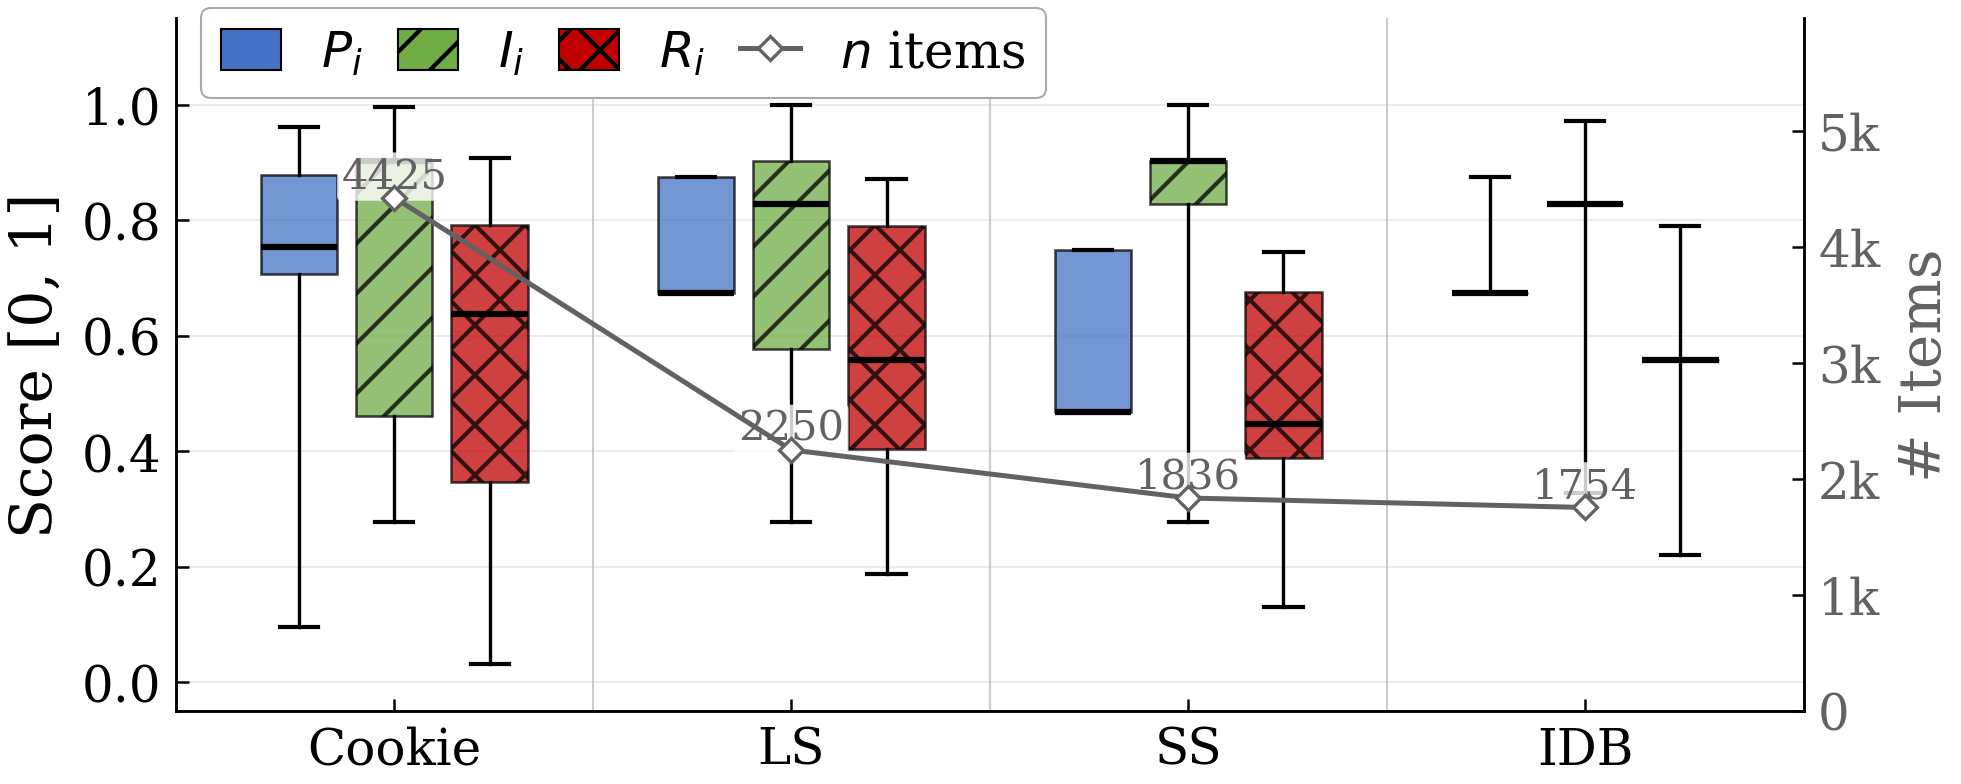
\includegraphics[width=\textwidth]{risk_analysis_PxI_countries/src/outputs/figures/f1_metrics_by_storage_AUTH_IE_0504_PARTIAL.png}
\caption{IE\_0504 -- AUTH}
\end{subfigure}\hfill
\begin{subfigure}{0.48\textwidth}
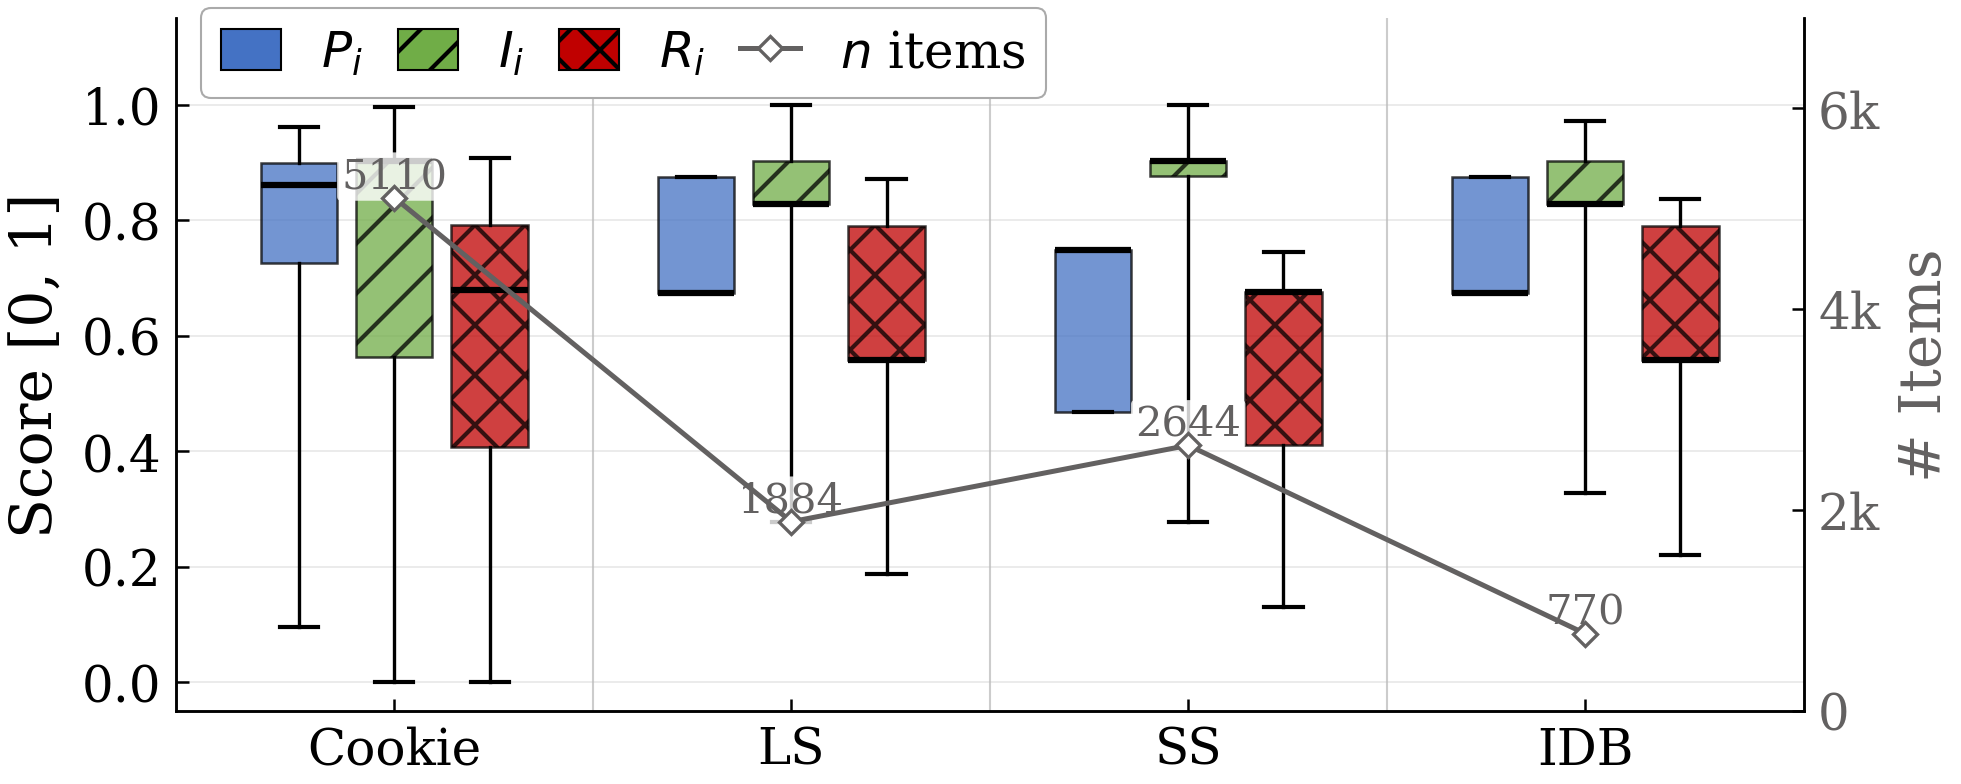
\includegraphics[width=\textwidth]{risk_analysis_PxI_countries/src/outputs/figures/f1_metrics_by_storage_NOTAUTH_IE_0504_PARTIAL.png}
\caption{IE\_0504 -- NOTAUTH}
\end{subfigure}
\end{figure}

\begin{figure}[h]
\centering
\begin{subfigure}{0.48\textwidth}
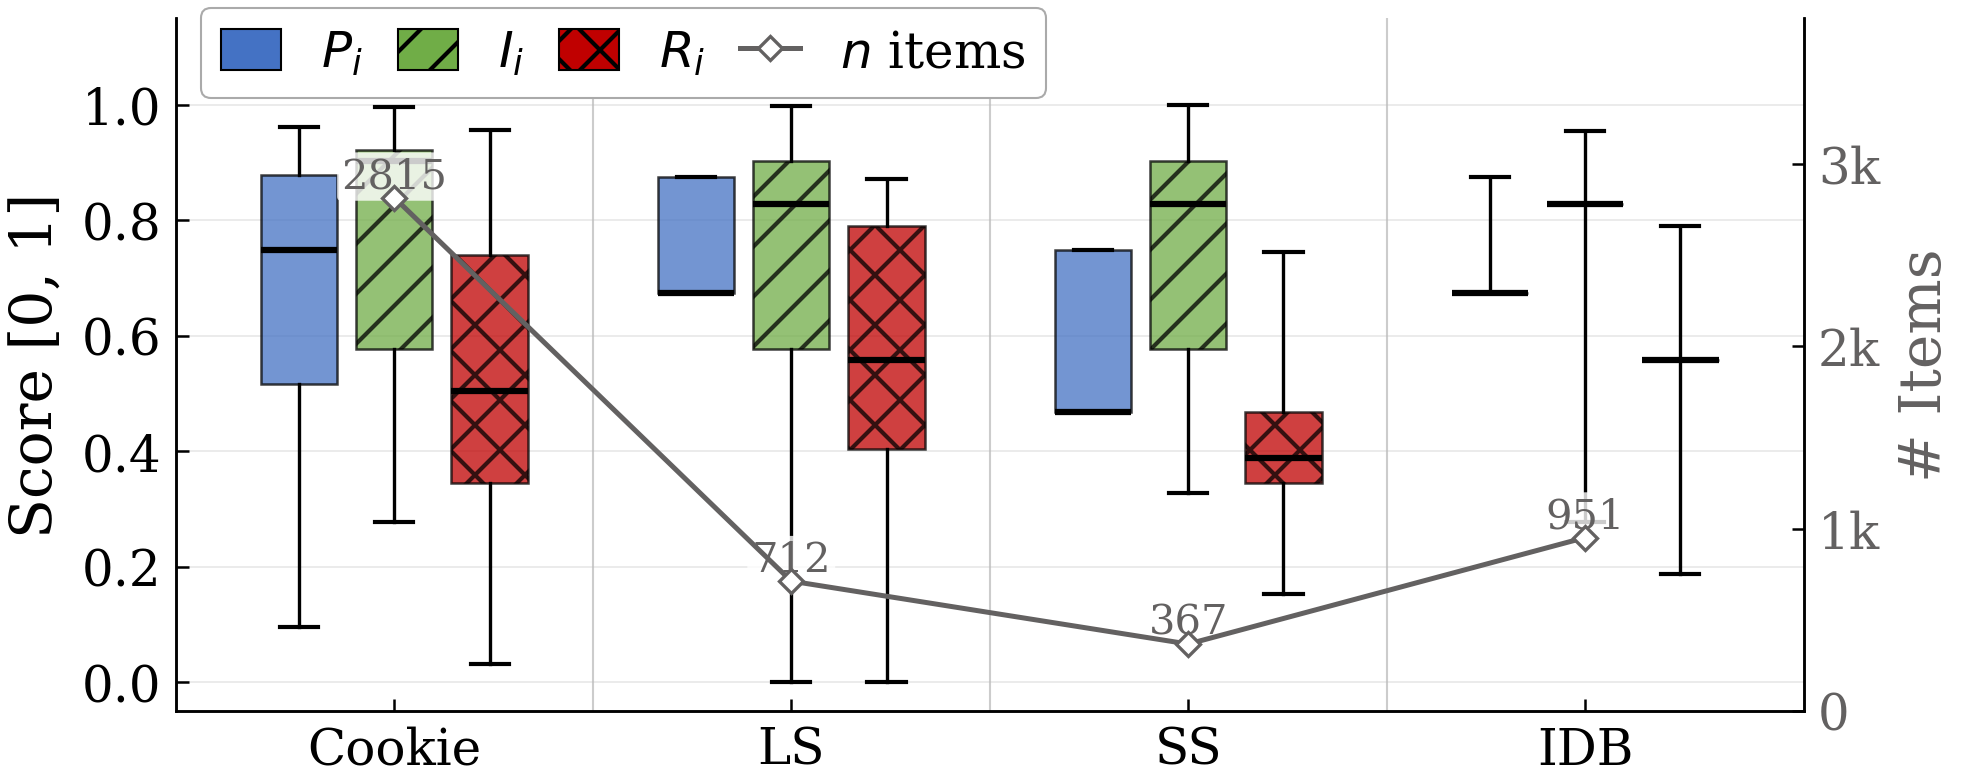
\includegraphics[width=\textwidth]{risk_analysis_PxI_countries/src/outputs/figures/f1_metrics_by_storage_AUTH_NL_0694_PARTIAL.png}
\caption{NL\_0694 -- AUTH}
\end{subfigure}\hfill
\begin{subfigure}{0.48\textwidth}
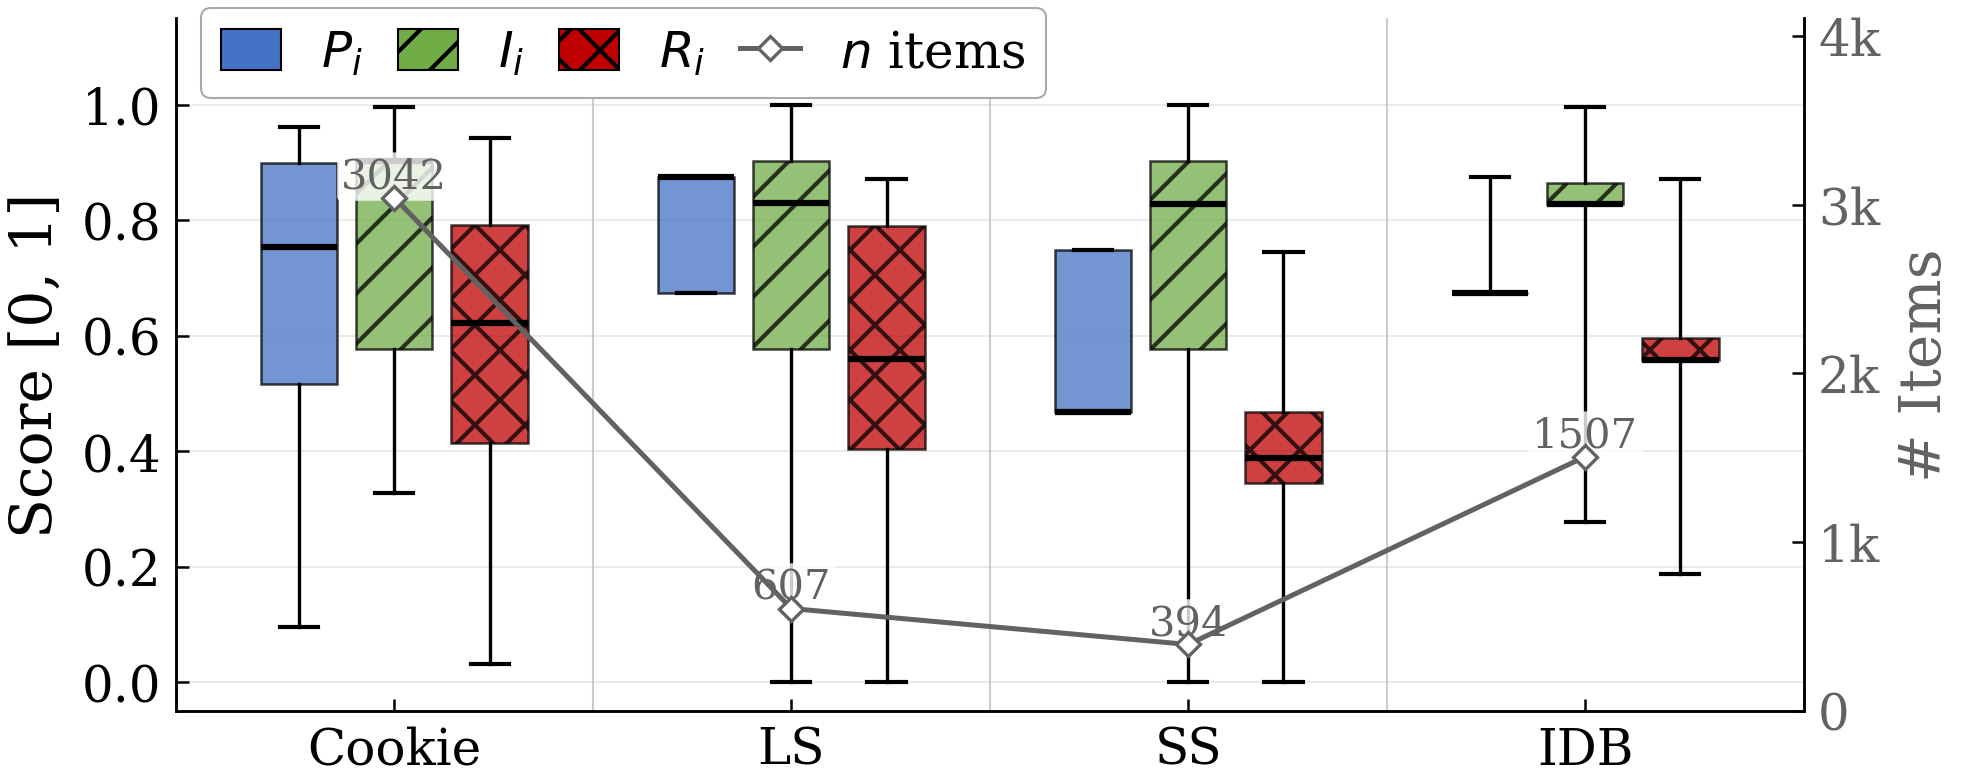
\includegraphics[width=\textwidth]{risk_analysis_PxI_countries/src/outputs/figures/f1_metrics_by_storage_NOTAUTH_NL_0694_PARTIAL.png}
\caption{NL\_0694 -- NOTAUTH}
\end{subfigure}
\end{figure}

\begin{figure}[h]
\centering
\begin{subfigure}{0.48\textwidth}
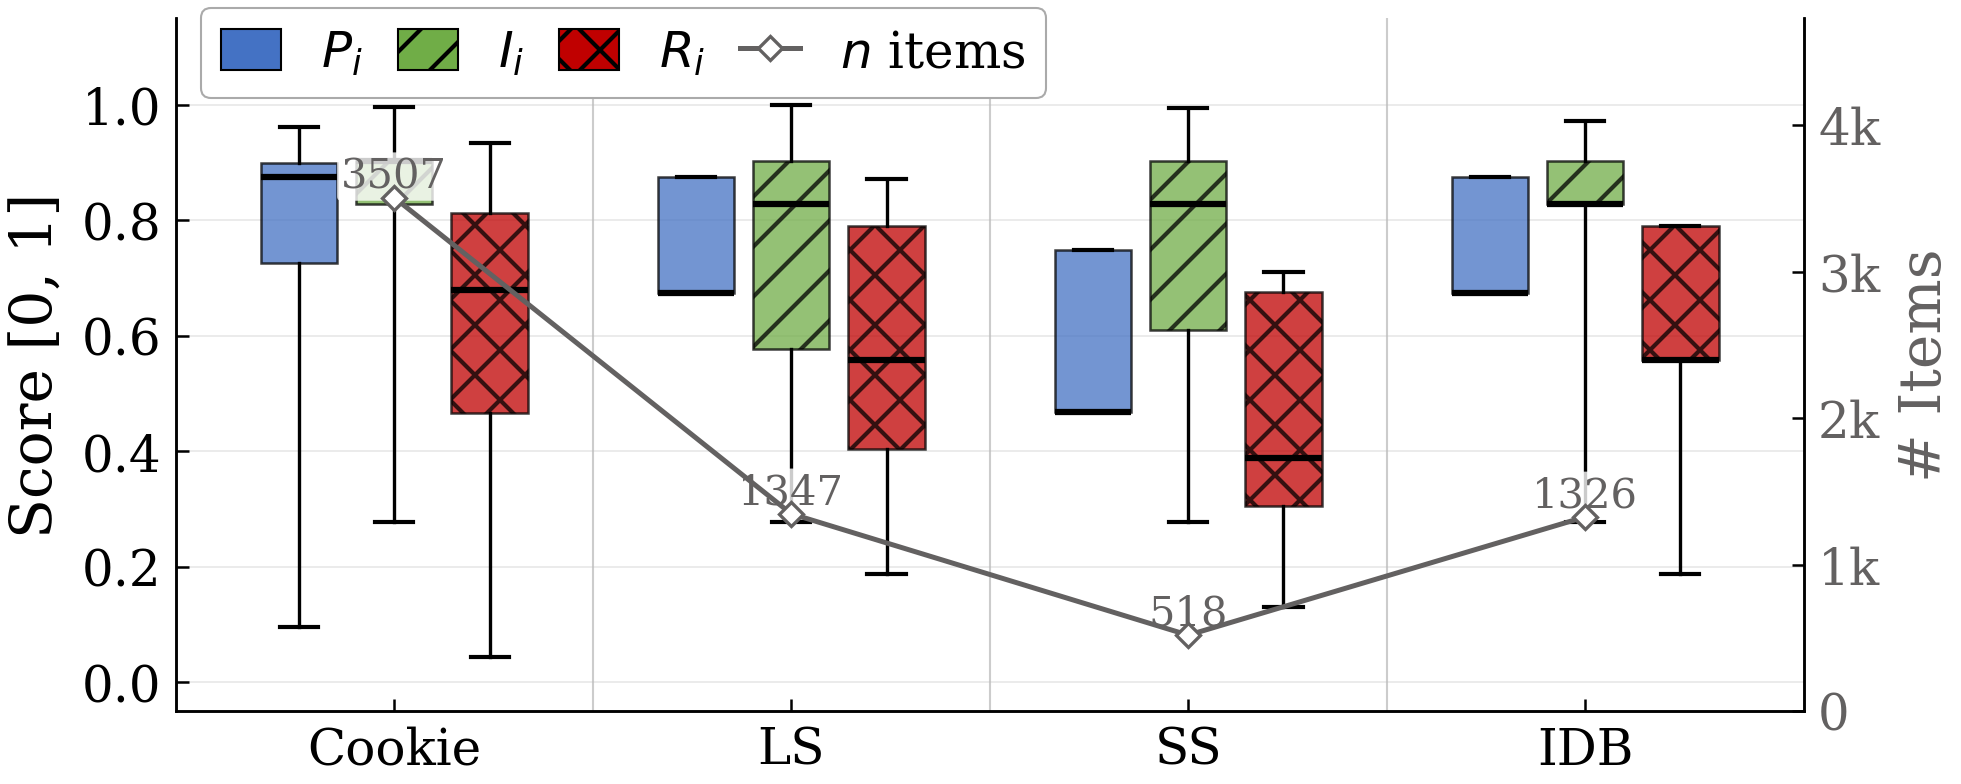
\includegraphics[width=\textwidth]{risk_analysis_PxI_countries/src/outputs/figures/f1_metrics_by_storage_AUTH_PL_0742_PARTIAL.png}
\caption{PL\_0742 -- AUTH}
\end{subfigure}\hfill
\begin{subfigure}{0.48\textwidth}
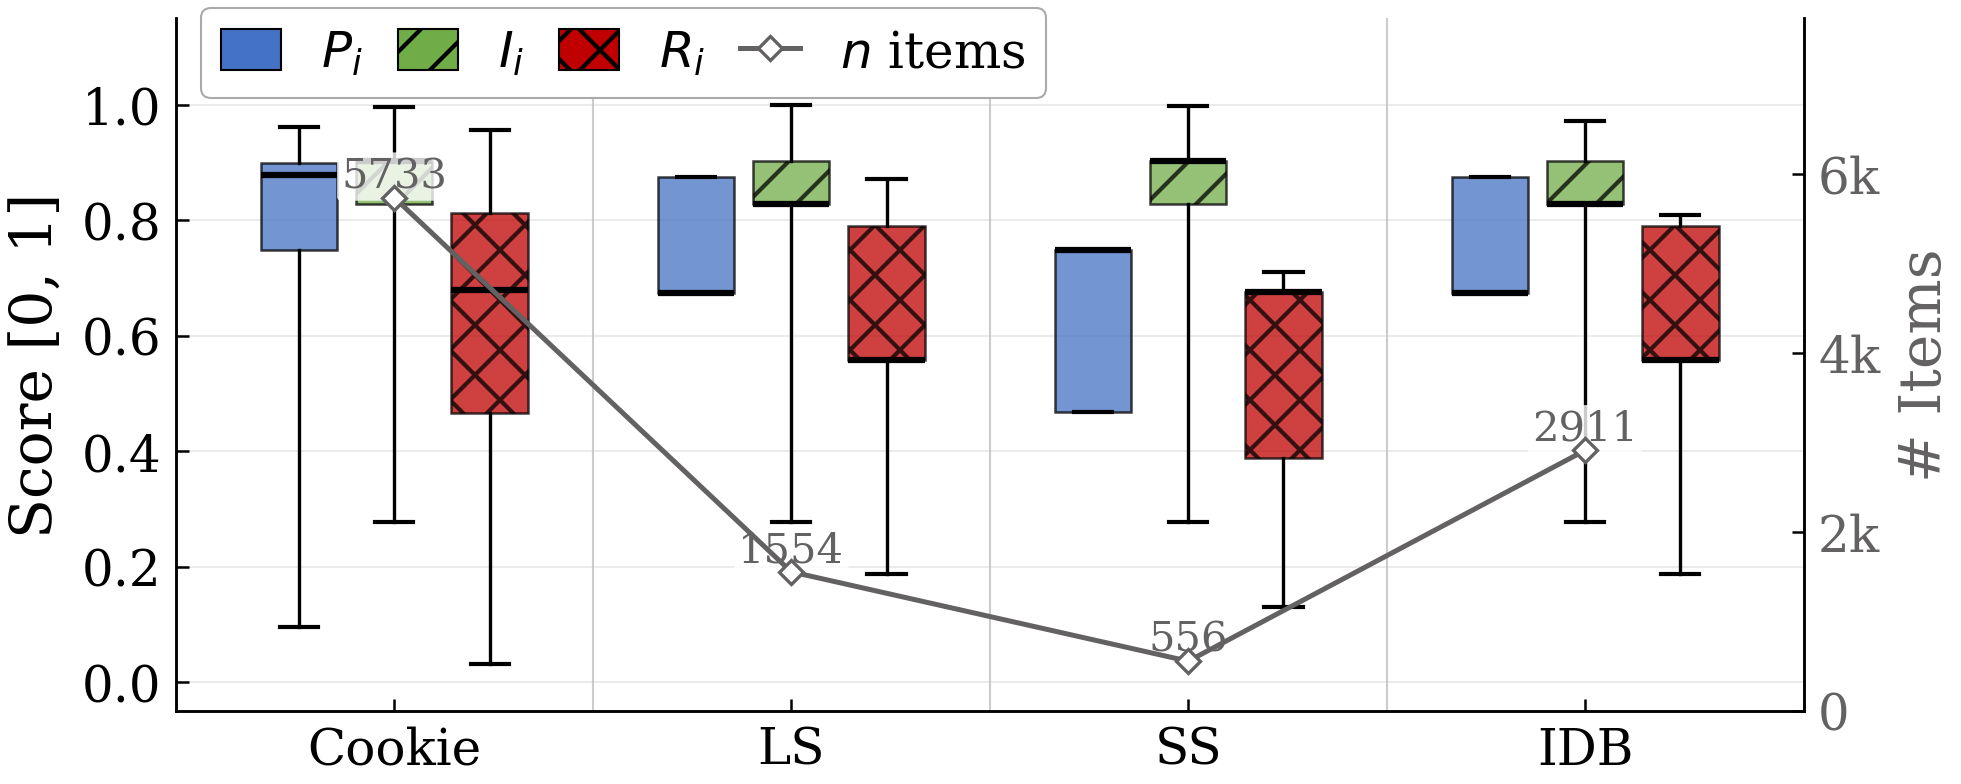
\includegraphics[width=\textwidth]{risk_analysis_PxI_countries/src/outputs/figures/f1_metrics_by_storage_NOTAUTH_PL_0742_PARTIAL.png}
\caption{PL\_0742 -- NOTAUTH}
\end{subfigure}
\end{figure}

\begin{figure}[h]
\centering
\begin{subfigure}{0.48\textwidth}
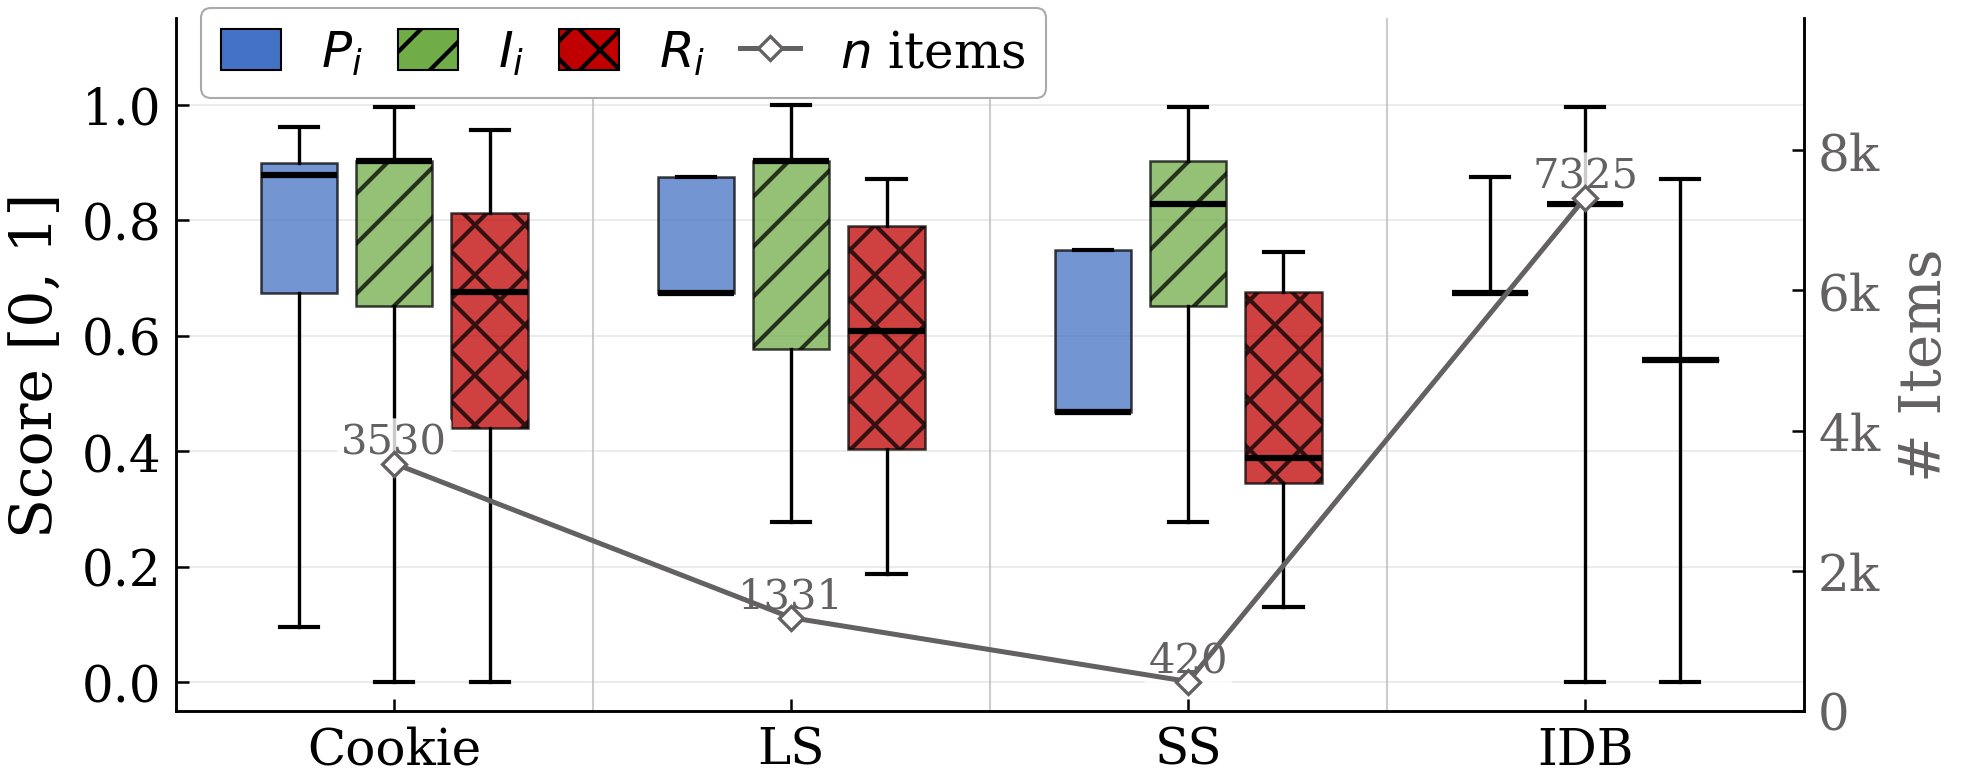
\includegraphics[width=\textwidth]{risk_analysis_PxI_countries/src/outputs/figures/f1_metrics_by_storage_AUTH_AT_0077_PARTIAL.png}
\caption{AT\_0077 -- AUTH}
\end{subfigure}\hfill
\begin{subfigure}{0.48\textwidth}
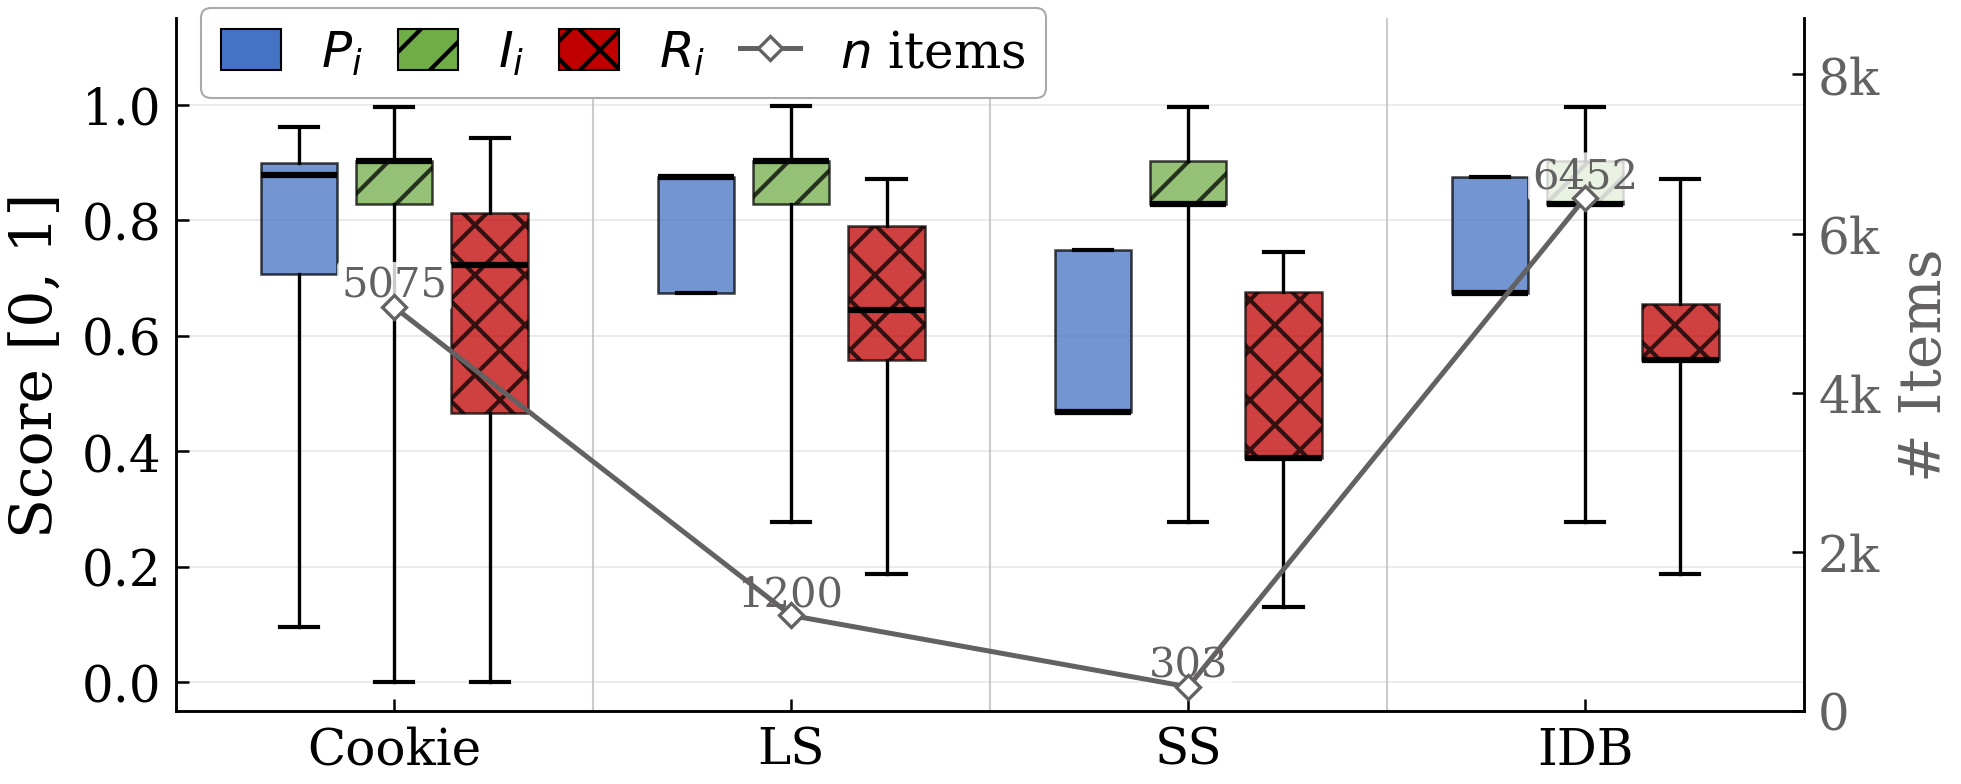
\includegraphics[width=\textwidth]{risk_analysis_PxI_countries/src/outputs/figures/f1_metrics_by_storage_NOTAUTH_AT_0077_PARTIAL.png}
\caption{AT\_0077 -- NOTAUTH}
\end{subfigure}
\end{figure}

\begin{figure}[h]
\centering
\begin{subfigure}{0.48\textwidth}
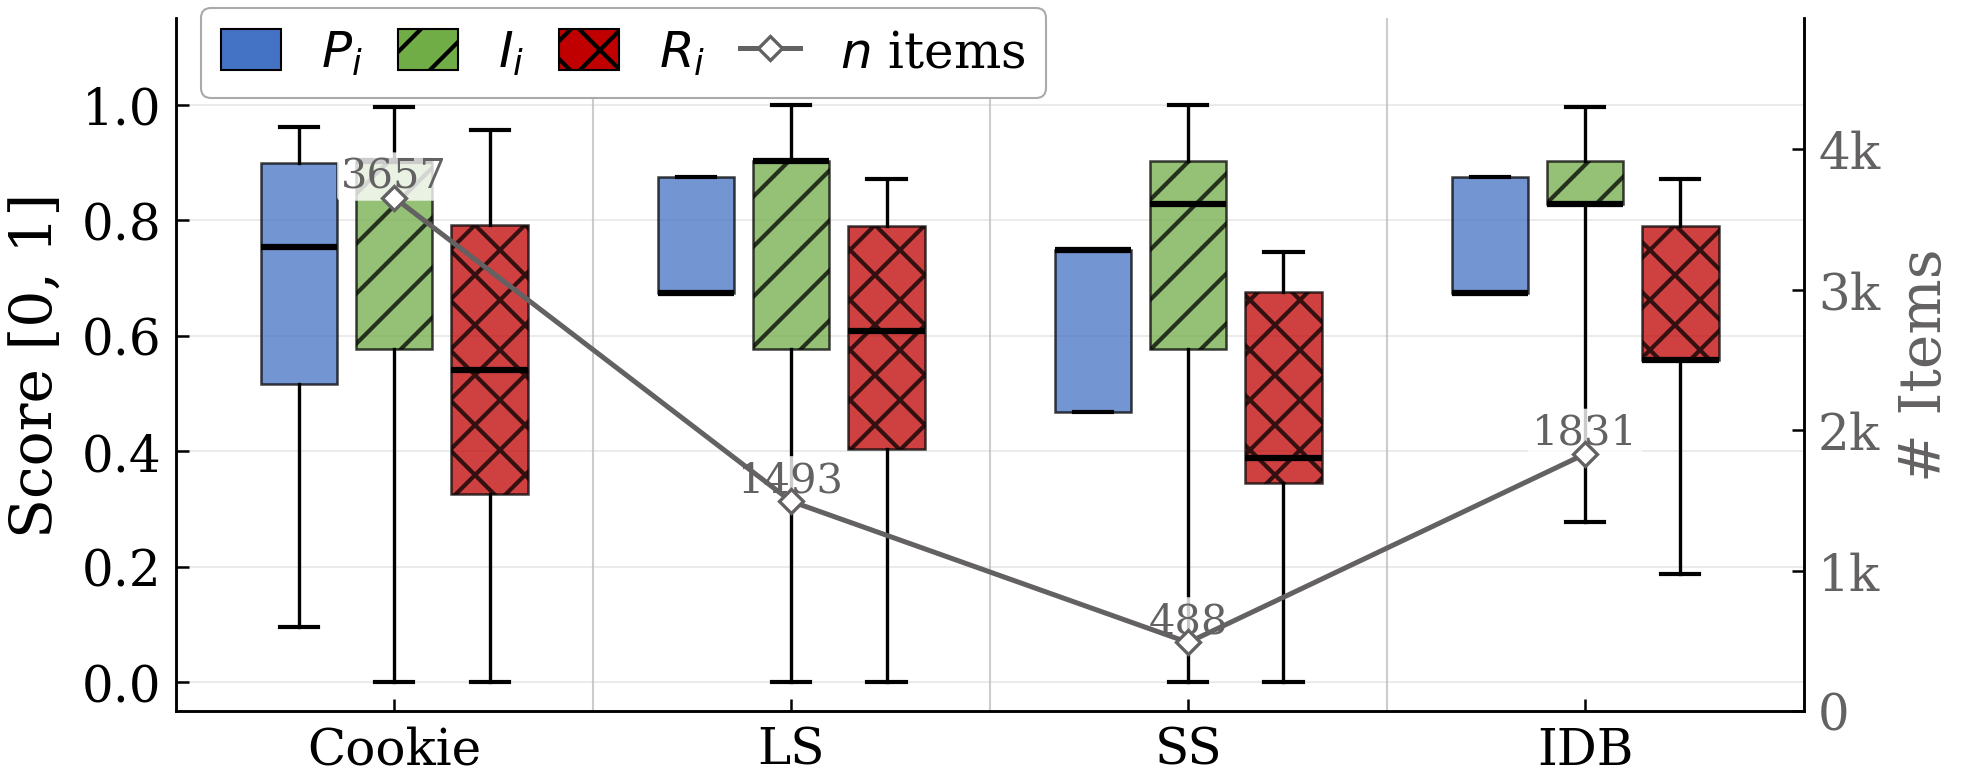
\includegraphics[width=\textwidth]{risk_analysis_PxI_countries/src/outputs/figures/f1_metrics_by_storage_AUTH_DK_0199_PARTIAL.png}
\caption{DK\_0199 -- AUTH}
\end{subfigure}\hfill
\begin{subfigure}{0.48\textwidth}
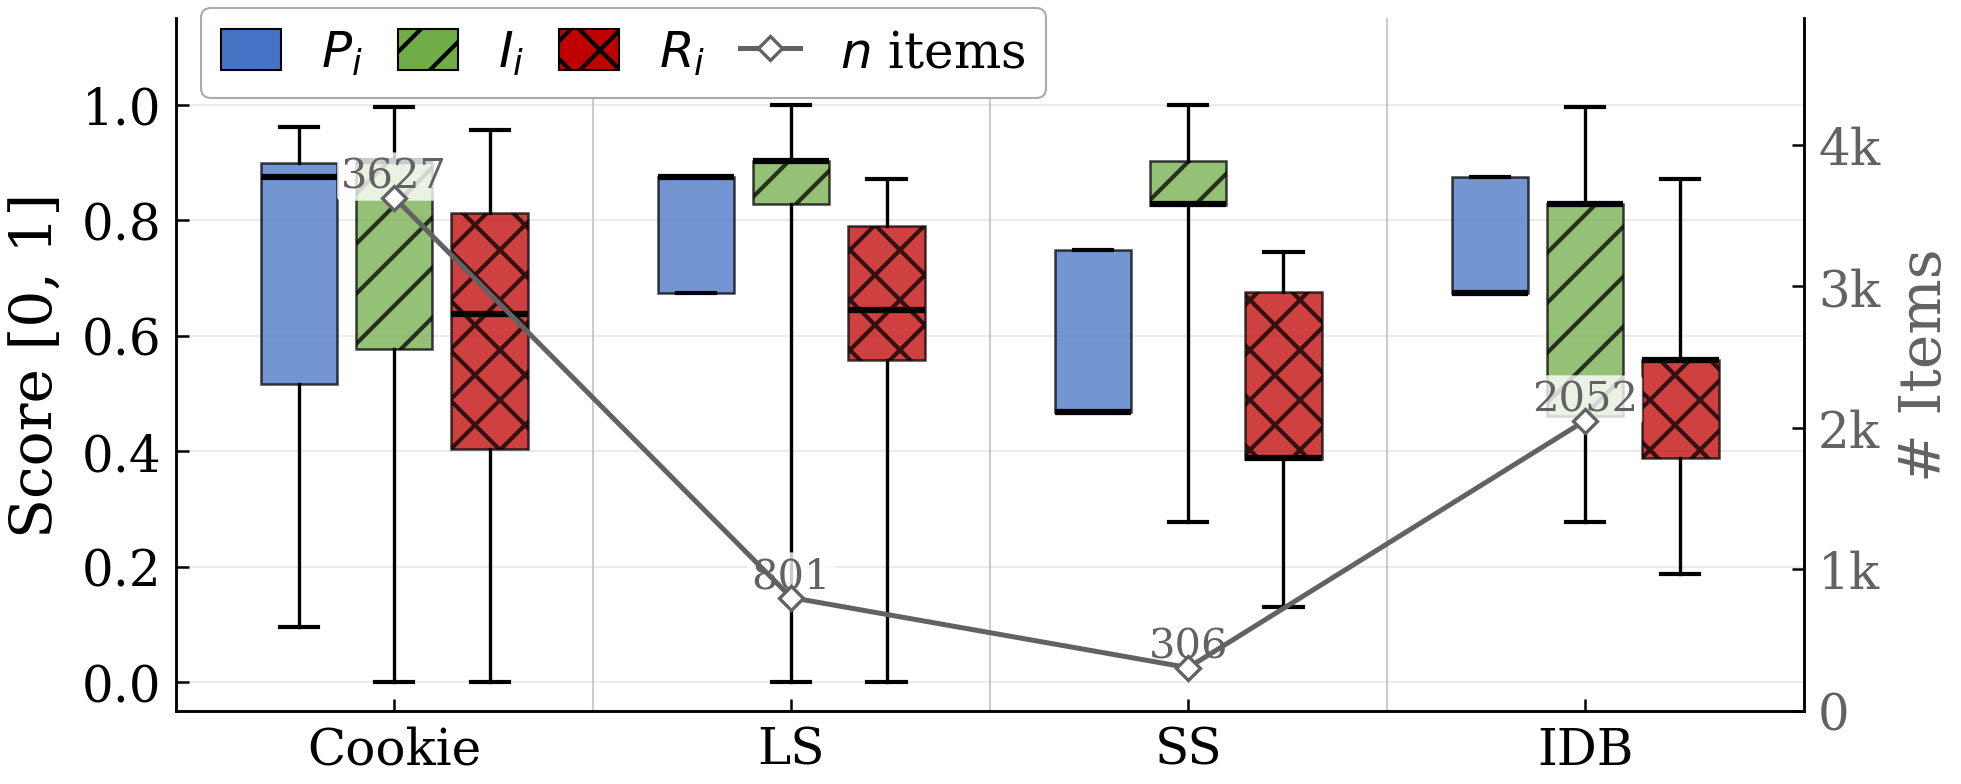
\includegraphics[width=\textwidth]{risk_analysis_PxI_countries/src/outputs/figures/f1_metrics_by_storage_NOTAUTH_DK_0199_PARTIAL.png}
\caption{DK\_0199 -- NOTAUTH}
\end{subfigure}
\end{figure}

\begin{figure}[h]
\centering
\begin{subfigure}{0.48\textwidth}
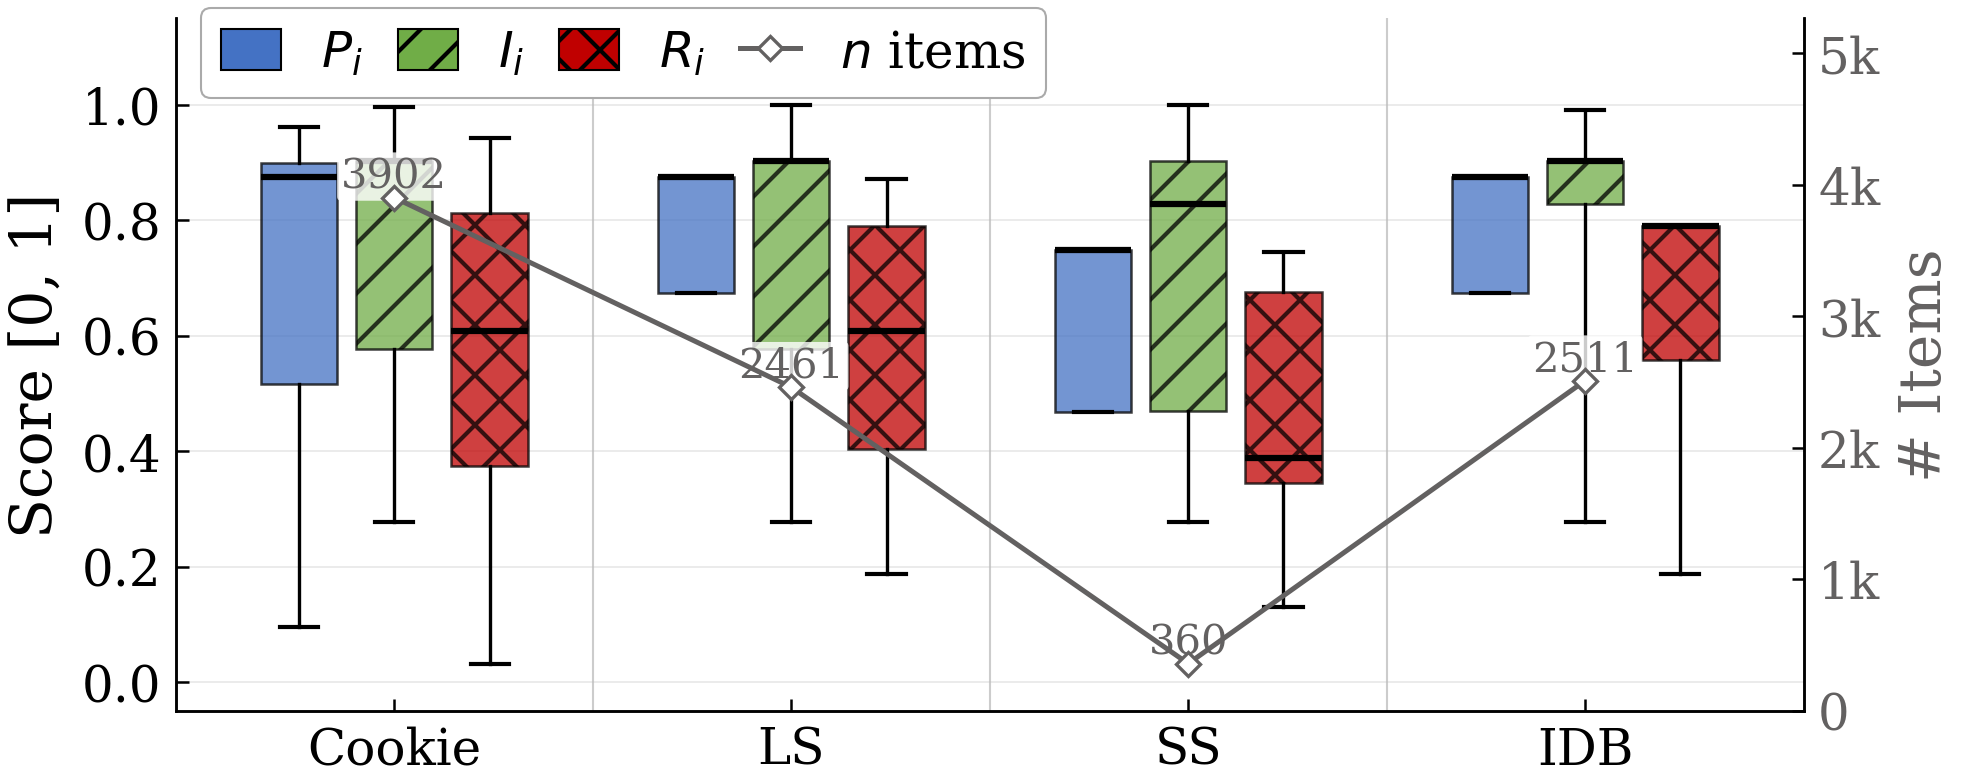
\includegraphics[width=\textwidth]{risk_analysis_PxI_countries/src/outputs/figures/f1_metrics_by_storage_AUTH_FI_0373_PARTIAL.png}
\caption{FI\_0373 -- AUTH}
\end{subfigure}\hfill
\begin{subfigure}{0.48\textwidth}
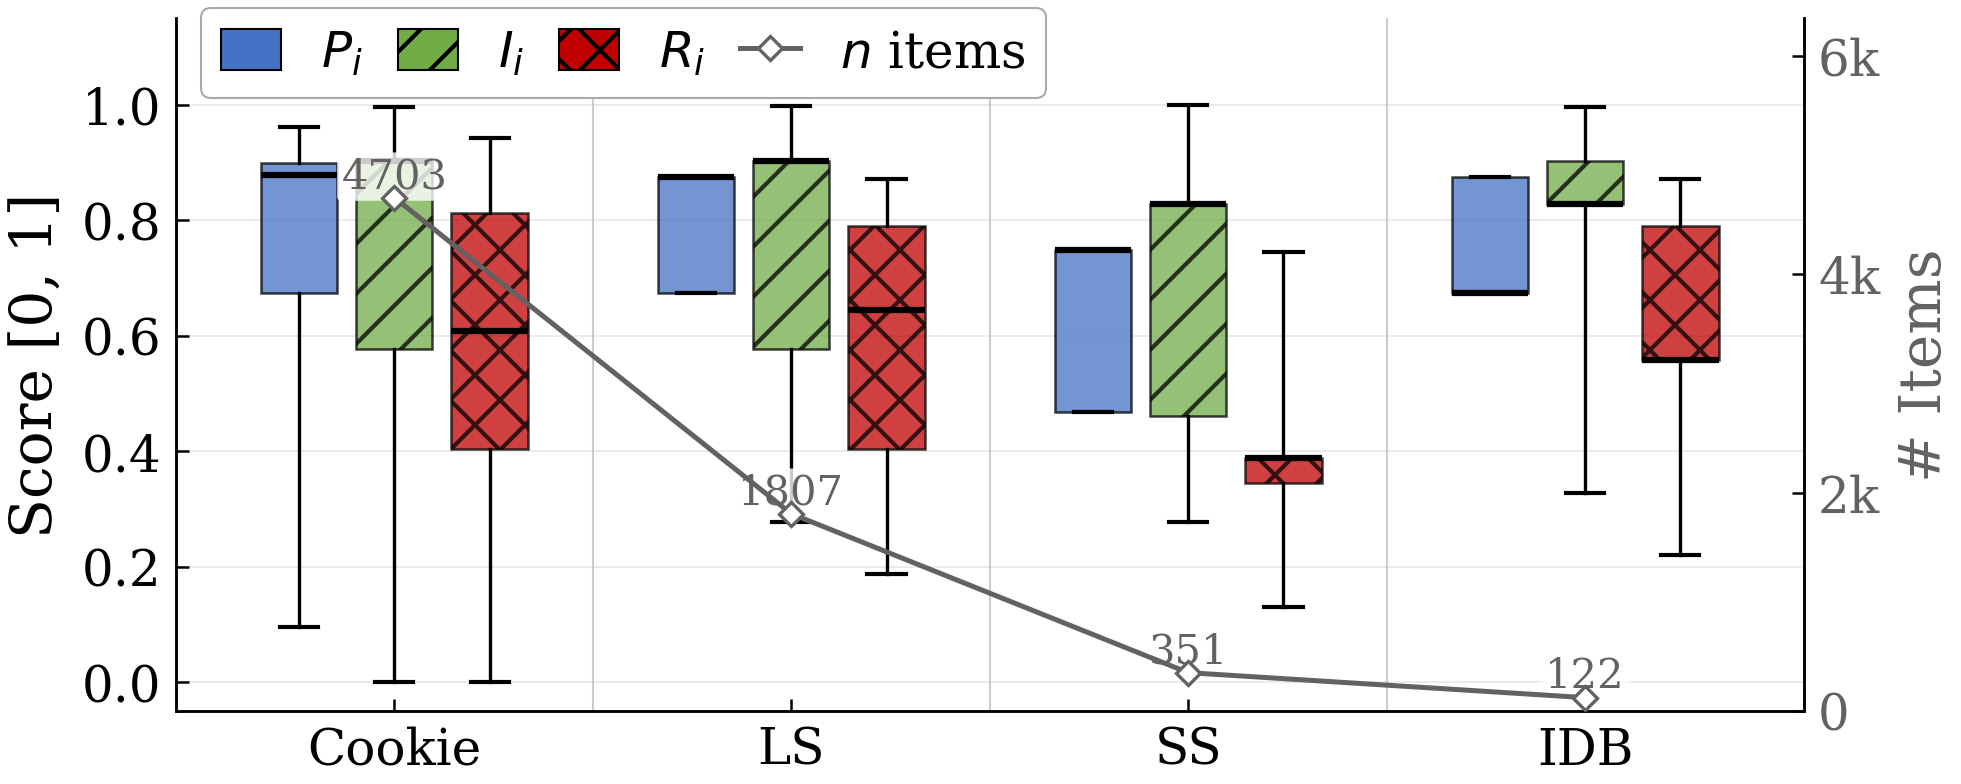
\includegraphics[width=\textwidth]{risk_analysis_PxI_countries/src/outputs/figures/f1_metrics_by_storage_NOTAUTH_FI_0373_PARTIAL.png}
\caption{FI\_0373 -- NOTAUTH}
\end{subfigure}
\end{figure}


\end{document}
